\documentclass[11pt]{article}

    \usepackage[breakable]{tcolorbox}
    \usepackage{parskip} % Stop auto-indenting (to mimic markdown behaviour)
    

    % Basic figure setup, for now with no caption control since it's done
    % automatically by Pandoc (which extracts ![](path) syntax from Markdown).
    \usepackage{graphicx}
    % Keep aspect ratio if custom image width or height is specified
    \setkeys{Gin}{keepaspectratio}
    % Maintain compatibility with old templates. Remove in nbconvert 6.0
    \let\Oldincludegraphics\includegraphics
    % Ensure that by default, figures have no caption (until we provide a
    % proper Figure object with a Caption API and a way to capture that
    % in the conversion process - todo).
    \usepackage{caption}
    \DeclareCaptionFormat{nocaption}{}
    \captionsetup{format=nocaption,aboveskip=0pt,belowskip=0pt}

    \usepackage{float}
    \floatplacement{figure}{H} % forces figures to be placed at the correct location
    \usepackage{xcolor} % Allow colors to be defined
    \usepackage{enumerate} % Needed for markdown enumerations to work
    \usepackage{geometry} % Used to adjust the document margins
    \usepackage{amsmath} % Equations
    \usepackage{amssymb} % Equations
    \usepackage{textcomp} % defines textquotesingle
    % Hack from http://tex.stackexchange.com/a/47451/13684:
    \AtBeginDocument{%
        \def\PYZsq{\textquotesingle}% Upright quotes in Pygmentized code
    }
    \usepackage{upquote} % Upright quotes for verbatim code
    \usepackage{eurosym} % defines \euro

    \usepackage{iftex}
    \ifPDFTeX
        \usepackage[T1]{fontenc}
        \IfFileExists{alphabeta.sty}{
              \usepackage{alphabeta}
          }{
              \usepackage[mathletters]{ucs}
              \usepackage[utf8x]{inputenc}
          }
    \else
        \usepackage{fontspec}
        \usepackage{unicode-math}
    \fi

    \usepackage{fancyvrb} % verbatim replacement that allows latex
    \usepackage{grffile} % extends the file name processing of package graphics
                         % to support a larger range
    \makeatletter % fix for old versions of grffile with XeLaTeX
    \@ifpackagelater{grffile}{2019/11/01}
    {
      % Do nothing on new versions
    }
    {
      \def\Gread@@xetex#1{%
        \IfFileExists{"\Gin@base".bb}%
        {\Gread@eps{\Gin@base.bb}}%
        {\Gread@@xetex@aux#1}%
      }
    }
    \makeatother
    \usepackage[Export]{adjustbox} % Used to constrain images to a maximum size
    \adjustboxset{max size={0.9\linewidth}{0.9\paperheight}}

    % The hyperref package gives us a pdf with properly built
    % internal navigation ('pdf bookmarks' for the table of contents,
    % internal cross-reference links, web links for URLs, etc.)
    \usepackage{hyperref}
    % The default LaTeX title has an obnoxious amount of whitespace. By default,
    % titling removes some of it. It also provides customization options.
    \usepackage{titling}
    \usepackage{longtable} % longtable support required by pandoc >1.10
    \usepackage{booktabs}  % table support for pandoc > 1.12.2
    \usepackage{array}     % table support for pandoc >= 2.11.3
    \usepackage{calc}      % table minipage width calculation for pandoc >= 2.11.1
    \usepackage[inline]{enumitem} % IRkernel/repr support (it uses the enumerate* environment)
    \usepackage[normalem]{ulem} % ulem is needed to support strikethroughs (\sout)
                                % normalem makes italics be italics, not underlines
    \usepackage{soul}      % strikethrough (\st) support for pandoc >= 3.0.0
    \usepackage{mathrsfs}
    

    
    % Colors for the hyperref package
    \definecolor{urlcolor}{rgb}{0,.145,.698}
    \definecolor{linkcolor}{rgb}{.71,0.21,0.01}
    \definecolor{citecolor}{rgb}{.12,.54,.11}

    % ANSI colors
    \definecolor{ansi-black}{HTML}{3E424D}
    \definecolor{ansi-black-intense}{HTML}{282C36}
    \definecolor{ansi-red}{HTML}{E75C58}
    \definecolor{ansi-red-intense}{HTML}{B22B31}
    \definecolor{ansi-green}{HTML}{00A250}
    \definecolor{ansi-green-intense}{HTML}{007427}
    \definecolor{ansi-yellow}{HTML}{DDB62B}
    \definecolor{ansi-yellow-intense}{HTML}{B27D12}
    \definecolor{ansi-blue}{HTML}{208FFB}
    \definecolor{ansi-blue-intense}{HTML}{0065CA}
    \definecolor{ansi-magenta}{HTML}{D160C4}
    \definecolor{ansi-magenta-intense}{HTML}{A03196}
    \definecolor{ansi-cyan}{HTML}{60C6C8}
    \definecolor{ansi-cyan-intense}{HTML}{258F8F}
    \definecolor{ansi-white}{HTML}{C5C1B4}
    \definecolor{ansi-white-intense}{HTML}{A1A6B2}
    \definecolor{ansi-default-inverse-fg}{HTML}{FFFFFF}
    \definecolor{ansi-default-inverse-bg}{HTML}{000000}

    % common color for the border for error outputs.
    \definecolor{outerrorbackground}{HTML}{FFDFDF}

    % commands and environments needed by pandoc snippets
    % extracted from the output of `pandoc -s`
    \providecommand{\tightlist}{%
      \setlength{\itemsep}{0pt}\setlength{\parskip}{0pt}}
    \DefineVerbatimEnvironment{Highlighting}{Verbatim}{commandchars=\\\{\}}
    % Add ',fontsize=\small' for more characters per line
    \newenvironment{Shaded}{}{}
    \newcommand{\KeywordTok}[1]{\textcolor[rgb]{0.00,0.44,0.13}{\textbf{{#1}}}}
    \newcommand{\DataTypeTok}[1]{\textcolor[rgb]{0.56,0.13,0.00}{{#1}}}
    \newcommand{\DecValTok}[1]{\textcolor[rgb]{0.25,0.63,0.44}{{#1}}}
    \newcommand{\BaseNTok}[1]{\textcolor[rgb]{0.25,0.63,0.44}{{#1}}}
    \newcommand{\FloatTok}[1]{\textcolor[rgb]{0.25,0.63,0.44}{{#1}}}
    \newcommand{\CharTok}[1]{\textcolor[rgb]{0.25,0.44,0.63}{{#1}}}
    \newcommand{\StringTok}[1]{\textcolor[rgb]{0.25,0.44,0.63}{{#1}}}
    \newcommand{\CommentTok}[1]{\textcolor[rgb]{0.38,0.63,0.69}{\textit{{#1}}}}
    \newcommand{\OtherTok}[1]{\textcolor[rgb]{0.00,0.44,0.13}{{#1}}}
    \newcommand{\AlertTok}[1]{\textcolor[rgb]{1.00,0.00,0.00}{\textbf{{#1}}}}
    \newcommand{\FunctionTok}[1]{\textcolor[rgb]{0.02,0.16,0.49}{{#1}}}
    \newcommand{\RegionMarkerTok}[1]{{#1}}
    \newcommand{\ErrorTok}[1]{\textcolor[rgb]{1.00,0.00,0.00}{\textbf{{#1}}}}
    \newcommand{\NormalTok}[1]{{#1}}

    % Additional commands for more recent versions of Pandoc
    \newcommand{\ConstantTok}[1]{\textcolor[rgb]{0.53,0.00,0.00}{{#1}}}
    \newcommand{\SpecialCharTok}[1]{\textcolor[rgb]{0.25,0.44,0.63}{{#1}}}
    \newcommand{\VerbatimStringTok}[1]{\textcolor[rgb]{0.25,0.44,0.63}{{#1}}}
    \newcommand{\SpecialStringTok}[1]{\textcolor[rgb]{0.73,0.40,0.53}{{#1}}}
    \newcommand{\ImportTok}[1]{{#1}}
    \newcommand{\DocumentationTok}[1]{\textcolor[rgb]{0.73,0.13,0.13}{\textit{{#1}}}}
    \newcommand{\AnnotationTok}[1]{\textcolor[rgb]{0.38,0.63,0.69}{\textbf{\textit{{#1}}}}}
    \newcommand{\CommentVarTok}[1]{\textcolor[rgb]{0.38,0.63,0.69}{\textbf{\textit{{#1}}}}}
    \newcommand{\VariableTok}[1]{\textcolor[rgb]{0.10,0.09,0.49}{{#1}}}
    \newcommand{\ControlFlowTok}[1]{\textcolor[rgb]{0.00,0.44,0.13}{\textbf{{#1}}}}
    \newcommand{\OperatorTok}[1]{\textcolor[rgb]{0.40,0.40,0.40}{{#1}}}
    \newcommand{\BuiltInTok}[1]{{#1}}
    \newcommand{\ExtensionTok}[1]{{#1}}
    \newcommand{\PreprocessorTok}[1]{\textcolor[rgb]{0.74,0.48,0.00}{{#1}}}
    \newcommand{\AttributeTok}[1]{\textcolor[rgb]{0.49,0.56,0.16}{{#1}}}
    \newcommand{\InformationTok}[1]{\textcolor[rgb]{0.38,0.63,0.69}{\textbf{\textit{{#1}}}}}
    \newcommand{\WarningTok}[1]{\textcolor[rgb]{0.38,0.63,0.69}{\textbf{\textit{{#1}}}}}


    % Define a nice break command that doesn't care if a line doesn't already
    % exist.
    \def\br{\hspace*{\fill} \\* }
    % Math Jax compatibility definitions
    \def\gt{>}
    \def\lt{<}
    \let\Oldtex\TeX
    \let\Oldlatex\LaTeX
    \renewcommand{\TeX}{\textrm{\Oldtex}}
    \renewcommand{\LaTeX}{\textrm{\Oldlatex}}
    % Document parameters
    % Document title
    \title{Assignment}
    
    
    
    
    
    
    
% Pygments definitions
\makeatletter
\def\PY@reset{\let\PY@it=\relax \let\PY@bf=\relax%
    \let\PY@ul=\relax \let\PY@tc=\relax%
    \let\PY@bc=\relax \let\PY@ff=\relax}
\def\PY@tok#1{\csname PY@tok@#1\endcsname}
\def\PY@toks#1+{\ifx\relax#1\empty\else%
    \PY@tok{#1}\expandafter\PY@toks\fi}
\def\PY@do#1{\PY@bc{\PY@tc{\PY@ul{%
    \PY@it{\PY@bf{\PY@ff{#1}}}}}}}
\def\PY#1#2{\PY@reset\PY@toks#1+\relax+\PY@do{#2}}

\@namedef{PY@tok@w}{\def\PY@tc##1{\textcolor[rgb]{0.73,0.73,0.73}{##1}}}
\@namedef{PY@tok@c}{\let\PY@it=\textit\def\PY@tc##1{\textcolor[rgb]{0.24,0.48,0.48}{##1}}}
\@namedef{PY@tok@cp}{\def\PY@tc##1{\textcolor[rgb]{0.61,0.40,0.00}{##1}}}
\@namedef{PY@tok@k}{\let\PY@bf=\textbf\def\PY@tc##1{\textcolor[rgb]{0.00,0.50,0.00}{##1}}}
\@namedef{PY@tok@kp}{\def\PY@tc##1{\textcolor[rgb]{0.00,0.50,0.00}{##1}}}
\@namedef{PY@tok@kt}{\def\PY@tc##1{\textcolor[rgb]{0.69,0.00,0.25}{##1}}}
\@namedef{PY@tok@o}{\def\PY@tc##1{\textcolor[rgb]{0.40,0.40,0.40}{##1}}}
\@namedef{PY@tok@ow}{\let\PY@bf=\textbf\def\PY@tc##1{\textcolor[rgb]{0.67,0.13,1.00}{##1}}}
\@namedef{PY@tok@nb}{\def\PY@tc##1{\textcolor[rgb]{0.00,0.50,0.00}{##1}}}
\@namedef{PY@tok@nf}{\def\PY@tc##1{\textcolor[rgb]{0.00,0.00,1.00}{##1}}}
\@namedef{PY@tok@nc}{\let\PY@bf=\textbf\def\PY@tc##1{\textcolor[rgb]{0.00,0.00,1.00}{##1}}}
\@namedef{PY@tok@nn}{\let\PY@bf=\textbf\def\PY@tc##1{\textcolor[rgb]{0.00,0.00,1.00}{##1}}}
\@namedef{PY@tok@ne}{\let\PY@bf=\textbf\def\PY@tc##1{\textcolor[rgb]{0.80,0.25,0.22}{##1}}}
\@namedef{PY@tok@nv}{\def\PY@tc##1{\textcolor[rgb]{0.10,0.09,0.49}{##1}}}
\@namedef{PY@tok@no}{\def\PY@tc##1{\textcolor[rgb]{0.53,0.00,0.00}{##1}}}
\@namedef{PY@tok@nl}{\def\PY@tc##1{\textcolor[rgb]{0.46,0.46,0.00}{##1}}}
\@namedef{PY@tok@ni}{\let\PY@bf=\textbf\def\PY@tc##1{\textcolor[rgb]{0.44,0.44,0.44}{##1}}}
\@namedef{PY@tok@na}{\def\PY@tc##1{\textcolor[rgb]{0.41,0.47,0.13}{##1}}}
\@namedef{PY@tok@nt}{\let\PY@bf=\textbf\def\PY@tc##1{\textcolor[rgb]{0.00,0.50,0.00}{##1}}}
\@namedef{PY@tok@nd}{\def\PY@tc##1{\textcolor[rgb]{0.67,0.13,1.00}{##1}}}
\@namedef{PY@tok@s}{\def\PY@tc##1{\textcolor[rgb]{0.73,0.13,0.13}{##1}}}
\@namedef{PY@tok@sd}{\let\PY@it=\textit\def\PY@tc##1{\textcolor[rgb]{0.73,0.13,0.13}{##1}}}
\@namedef{PY@tok@si}{\let\PY@bf=\textbf\def\PY@tc##1{\textcolor[rgb]{0.64,0.35,0.47}{##1}}}
\@namedef{PY@tok@se}{\let\PY@bf=\textbf\def\PY@tc##1{\textcolor[rgb]{0.67,0.36,0.12}{##1}}}
\@namedef{PY@tok@sr}{\def\PY@tc##1{\textcolor[rgb]{0.64,0.35,0.47}{##1}}}
\@namedef{PY@tok@ss}{\def\PY@tc##1{\textcolor[rgb]{0.10,0.09,0.49}{##1}}}
\@namedef{PY@tok@sx}{\def\PY@tc##1{\textcolor[rgb]{0.00,0.50,0.00}{##1}}}
\@namedef{PY@tok@m}{\def\PY@tc##1{\textcolor[rgb]{0.40,0.40,0.40}{##1}}}
\@namedef{PY@tok@gh}{\let\PY@bf=\textbf\def\PY@tc##1{\textcolor[rgb]{0.00,0.00,0.50}{##1}}}
\@namedef{PY@tok@gu}{\let\PY@bf=\textbf\def\PY@tc##1{\textcolor[rgb]{0.50,0.00,0.50}{##1}}}
\@namedef{PY@tok@gd}{\def\PY@tc##1{\textcolor[rgb]{0.63,0.00,0.00}{##1}}}
\@namedef{PY@tok@gi}{\def\PY@tc##1{\textcolor[rgb]{0.00,0.52,0.00}{##1}}}
\@namedef{PY@tok@gr}{\def\PY@tc##1{\textcolor[rgb]{0.89,0.00,0.00}{##1}}}
\@namedef{PY@tok@ge}{\let\PY@it=\textit}
\@namedef{PY@tok@gs}{\let\PY@bf=\textbf}
\@namedef{PY@tok@ges}{\let\PY@bf=\textbf\let\PY@it=\textit}
\@namedef{PY@tok@gp}{\let\PY@bf=\textbf\def\PY@tc##1{\textcolor[rgb]{0.00,0.00,0.50}{##1}}}
\@namedef{PY@tok@go}{\def\PY@tc##1{\textcolor[rgb]{0.44,0.44,0.44}{##1}}}
\@namedef{PY@tok@gt}{\def\PY@tc##1{\textcolor[rgb]{0.00,0.27,0.87}{##1}}}
\@namedef{PY@tok@err}{\def\PY@bc##1{{\setlength{\fboxsep}{\string -\fboxrule}\fcolorbox[rgb]{1.00,0.00,0.00}{1,1,1}{\strut ##1}}}}
\@namedef{PY@tok@kc}{\let\PY@bf=\textbf\def\PY@tc##1{\textcolor[rgb]{0.00,0.50,0.00}{##1}}}
\@namedef{PY@tok@kd}{\let\PY@bf=\textbf\def\PY@tc##1{\textcolor[rgb]{0.00,0.50,0.00}{##1}}}
\@namedef{PY@tok@kn}{\let\PY@bf=\textbf\def\PY@tc##1{\textcolor[rgb]{0.00,0.50,0.00}{##1}}}
\@namedef{PY@tok@kr}{\let\PY@bf=\textbf\def\PY@tc##1{\textcolor[rgb]{0.00,0.50,0.00}{##1}}}
\@namedef{PY@tok@bp}{\def\PY@tc##1{\textcolor[rgb]{0.00,0.50,0.00}{##1}}}
\@namedef{PY@tok@fm}{\def\PY@tc##1{\textcolor[rgb]{0.00,0.00,1.00}{##1}}}
\@namedef{PY@tok@vc}{\def\PY@tc##1{\textcolor[rgb]{0.10,0.09,0.49}{##1}}}
\@namedef{PY@tok@vg}{\def\PY@tc##1{\textcolor[rgb]{0.10,0.09,0.49}{##1}}}
\@namedef{PY@tok@vi}{\def\PY@tc##1{\textcolor[rgb]{0.10,0.09,0.49}{##1}}}
\@namedef{PY@tok@vm}{\def\PY@tc##1{\textcolor[rgb]{0.10,0.09,0.49}{##1}}}
\@namedef{PY@tok@sa}{\def\PY@tc##1{\textcolor[rgb]{0.73,0.13,0.13}{##1}}}
\@namedef{PY@tok@sb}{\def\PY@tc##1{\textcolor[rgb]{0.73,0.13,0.13}{##1}}}
\@namedef{PY@tok@sc}{\def\PY@tc##1{\textcolor[rgb]{0.73,0.13,0.13}{##1}}}
\@namedef{PY@tok@dl}{\def\PY@tc##1{\textcolor[rgb]{0.73,0.13,0.13}{##1}}}
\@namedef{PY@tok@s2}{\def\PY@tc##1{\textcolor[rgb]{0.73,0.13,0.13}{##1}}}
\@namedef{PY@tok@sh}{\def\PY@tc##1{\textcolor[rgb]{0.73,0.13,0.13}{##1}}}
\@namedef{PY@tok@s1}{\def\PY@tc##1{\textcolor[rgb]{0.73,0.13,0.13}{##1}}}
\@namedef{PY@tok@mb}{\def\PY@tc##1{\textcolor[rgb]{0.40,0.40,0.40}{##1}}}
\@namedef{PY@tok@mf}{\def\PY@tc##1{\textcolor[rgb]{0.40,0.40,0.40}{##1}}}
\@namedef{PY@tok@mh}{\def\PY@tc##1{\textcolor[rgb]{0.40,0.40,0.40}{##1}}}
\@namedef{PY@tok@mi}{\def\PY@tc##1{\textcolor[rgb]{0.40,0.40,0.40}{##1}}}
\@namedef{PY@tok@il}{\def\PY@tc##1{\textcolor[rgb]{0.40,0.40,0.40}{##1}}}
\@namedef{PY@tok@mo}{\def\PY@tc##1{\textcolor[rgb]{0.40,0.40,0.40}{##1}}}
\@namedef{PY@tok@ch}{\let\PY@it=\textit\def\PY@tc##1{\textcolor[rgb]{0.24,0.48,0.48}{##1}}}
\@namedef{PY@tok@cm}{\let\PY@it=\textit\def\PY@tc##1{\textcolor[rgb]{0.24,0.48,0.48}{##1}}}
\@namedef{PY@tok@cpf}{\let\PY@it=\textit\def\PY@tc##1{\textcolor[rgb]{0.24,0.48,0.48}{##1}}}
\@namedef{PY@tok@c1}{\let\PY@it=\textit\def\PY@tc##1{\textcolor[rgb]{0.24,0.48,0.48}{##1}}}
\@namedef{PY@tok@cs}{\let\PY@it=\textit\def\PY@tc##1{\textcolor[rgb]{0.24,0.48,0.48}{##1}}}

\def\PYZbs{\char`\\}
\def\PYZus{\char`\_}
\def\PYZob{\char`\{}
\def\PYZcb{\char`\}}
\def\PYZca{\char`\^}
\def\PYZam{\char`\&}
\def\PYZlt{\char`\<}
\def\PYZgt{\char`\>}
\def\PYZsh{\char`\#}
\def\PYZpc{\char`\%}
\def\PYZdl{\char`\$}
\def\PYZhy{\char`\-}
\def\PYZsq{\char`\'}
\def\PYZdq{\char`\"}
\def\PYZti{\char`\~}
% for compatibility with earlier versions
\def\PYZat{@}
\def\PYZlb{[}
\def\PYZrb{]}
\makeatother


    % For linebreaks inside Verbatim environment from package fancyvrb.
    \makeatletter
        \newbox\Wrappedcontinuationbox
        \newbox\Wrappedvisiblespacebox
        \newcommand*\Wrappedvisiblespace {\textcolor{red}{\textvisiblespace}}
        \newcommand*\Wrappedcontinuationsymbol {\textcolor{red}{\llap{\tiny$\m@th\hookrightarrow$}}}
        \newcommand*\Wrappedcontinuationindent {3ex }
        \newcommand*\Wrappedafterbreak {\kern\Wrappedcontinuationindent\copy\Wrappedcontinuationbox}
        % Take advantage of the already applied Pygments mark-up to insert
        % potential linebreaks for TeX processing.
        %        {, <, #, %, $, ' and ": go to next line.
        %        _, }, ^, &, >, - and ~: stay at end of broken line.
        % Use of \textquotesingle for straight quote.
        \newcommand*\Wrappedbreaksatspecials {%
            \def\PYGZus{\discretionary{\char`\_}{\Wrappedafterbreak}{\char`\_}}%
            \def\PYGZob{\discretionary{}{\Wrappedafterbreak\char`\{}{\char`\{}}%
            \def\PYGZcb{\discretionary{\char`\}}{\Wrappedafterbreak}{\char`\}}}%
            \def\PYGZca{\discretionary{\char`\^}{\Wrappedafterbreak}{\char`\^}}%
            \def\PYGZam{\discretionary{\char`\&}{\Wrappedafterbreak}{\char`\&}}%
            \def\PYGZlt{\discretionary{}{\Wrappedafterbreak\char`\<}{\char`\<}}%
            \def\PYGZgt{\discretionary{\char`\>}{\Wrappedafterbreak}{\char`\>}}%
            \def\PYGZsh{\discretionary{}{\Wrappedafterbreak\char`\#}{\char`\#}}%
            \def\PYGZpc{\discretionary{}{\Wrappedafterbreak\char`\%}{\char`\%}}%
            \def\PYGZdl{\discretionary{}{\Wrappedafterbreak\char`\$}{\char`\$}}%
            \def\PYGZhy{\discretionary{\char`\-}{\Wrappedafterbreak}{\char`\-}}%
            \def\PYGZsq{\discretionary{}{\Wrappedafterbreak\textquotesingle}{\textquotesingle}}%
            \def\PYGZdq{\discretionary{}{\Wrappedafterbreak\char`\"}{\char`\"}}%
            \def\PYGZti{\discretionary{\char`\~}{\Wrappedafterbreak}{\char`\~}}%
        }
        % Some characters . , ; ? ! / are not pygmentized.
        % This macro makes them "active" and they will insert potential linebreaks
        \newcommand*\Wrappedbreaksatpunct {%
            \lccode`\~`\.\lowercase{\def~}{\discretionary{\hbox{\char`\.}}{\Wrappedafterbreak}{\hbox{\char`\.}}}%
            \lccode`\~`\,\lowercase{\def~}{\discretionary{\hbox{\char`\,}}{\Wrappedafterbreak}{\hbox{\char`\,}}}%
            \lccode`\~`\;\lowercase{\def~}{\discretionary{\hbox{\char`\;}}{\Wrappedafterbreak}{\hbox{\char`\;}}}%
            \lccode`\~`\:\lowercase{\def~}{\discretionary{\hbox{\char`\:}}{\Wrappedafterbreak}{\hbox{\char`\:}}}%
            \lccode`\~`\?\lowercase{\def~}{\discretionary{\hbox{\char`\?}}{\Wrappedafterbreak}{\hbox{\char`\?}}}%
            \lccode`\~`\!\lowercase{\def~}{\discretionary{\hbox{\char`\!}}{\Wrappedafterbreak}{\hbox{\char`\!}}}%
            \lccode`\~`\/\lowercase{\def~}{\discretionary{\hbox{\char`\/}}{\Wrappedafterbreak}{\hbox{\char`\/}}}%
            \catcode`\.\active
            \catcode`\,\active
            \catcode`\;\active
            \catcode`\:\active
            \catcode`\?\active
            \catcode`\!\active
            \catcode`\/\active
            \lccode`\~`\~
        }
    \makeatother

    \let\OriginalVerbatim=\Verbatim
    \makeatletter
    \renewcommand{\Verbatim}[1][1]{%
        %\parskip\z@skip
        \sbox\Wrappedcontinuationbox {\Wrappedcontinuationsymbol}%
        \sbox\Wrappedvisiblespacebox {\FV@SetupFont\Wrappedvisiblespace}%
        \def\FancyVerbFormatLine ##1{\hsize\linewidth
            \vtop{\raggedright\hyphenpenalty\z@\exhyphenpenalty\z@
                \doublehyphendemerits\z@\finalhyphendemerits\z@
                \strut ##1\strut}%
        }%
        % If the linebreak is at a space, the latter will be displayed as visible
        % space at end of first line, and a continuation symbol starts next line.
        % Stretch/shrink are however usually zero for typewriter font.
        \def\FV@Space {%
            \nobreak\hskip\z@ plus\fontdimen3\font minus\fontdimen4\font
            \discretionary{\copy\Wrappedvisiblespacebox}{\Wrappedafterbreak}
            {\kern\fontdimen2\font}%
        }%

        % Allow breaks at special characters using \PYG... macros.
        \Wrappedbreaksatspecials
        % Breaks at punctuation characters . , ; ? ! and / need catcode=\active
        \OriginalVerbatim[#1,codes*=\Wrappedbreaksatpunct]%
    }
    \makeatother

    % Exact colors from NB
    \definecolor{incolor}{HTML}{303F9F}
    \definecolor{outcolor}{HTML}{D84315}
    \definecolor{cellborder}{HTML}{CFCFCF}
    \definecolor{cellbackground}{HTML}{F7F7F7}

    % prompt
    \makeatletter
    \newcommand{\boxspacing}{\kern\kvtcb@left@rule\kern\kvtcb@boxsep}
    \makeatother
    \newcommand{\prompt}[4]{
        {\ttfamily\llap{{\color{#2}[#3]:\hspace{3pt}#4}}\vspace{-\baselineskip}}
    }
    

    
    % Prevent overflowing lines due to hard-to-break entities
    \sloppy
    % Setup hyperref package
    \hypersetup{
      breaklinks=true,  % so long urls are correctly broken across lines
      colorlinks=true,
      urlcolor=urlcolor,
      linkcolor=linkcolor,
      citecolor=citecolor,
      }
    % Slightly bigger margins than the latex defaults
    
    \geometry{verbose,tmargin=1in,bmargin=1in,lmargin=1in,rmargin=1in}
    
    

\begin{document}
    
    \maketitle
    
    

    
    \section{A* Algorithm}\label{a-algorithm}

\subsection{Preamble (Vishal Thomas
124108347)}\label{preamble-vishal-thomas-124108347}

\textbf{A*} is a heuristic search algorithm for increasing the
efficiency of Dijkstra's algorithm for pathfinding and graph traversal.
Here heuristic information means to find a suitable or an intuitive
function that helps us to find the shortest path between 2 nodes in a
graph, efficiently. It is used in gaming applications especially to
design the movements of agents when they are aiming to reach a goal. It
is used in network connection systems for sending packets between
routers, cost effectively. It also helps robots in navigation\(^{[1]}\).
It uses the heuristic cost of greedy best first search algorithm and
exact cost of Dijkstra's algorithm to find the shortest path. It
calculates the heuristic distance from node \textbf{n} to the end node
and exact cost from start node to \textbf{n}.

\(Distance_{new}(start,v) = Heuristic(v,end) + Distance_{old}(start,v)\)

\(Distance_{new}(start,v)\) is the new updated distance between start
node and node \textbf{v}, \(Distance_{old}(start,v)\) is the exact cost
of reaching node \textbf{v} from start node and \(Heuristic(v,end)\) is
the heuristic cost of reaching to end node from \textbf{v}. After
updating the distance in the graph, we will calculate the shortest path.

Navigation through Maps

For finding optimal path between 2 cities or places, we can use A*
search algorithm to calculate the shortest path between them. Here the
heuristic function could be the air distance(euclidean distance) or
great-circle distance between 2 cities.\(^{[2]}\)

Video Games

Pathfinding is a crucial part in Video Games. A* is one of the widely
used algorithms in games especially when it involves path-finding
problems such as moving characters from one grid point to another grid
point. Due to the exponential growth in complexity of the games,
researchers focused on improving the A* algorithm to meet the demands of
modern games. Many of the optimizations include improving heuristic
functions, search space(maps), data structures and reducing space
complexity.\(^{[3]}\)

    \subsection{Short history (Daniel Sedlov
123120712)}\label{short-history-daniel-sedlov-123120712}

The A* Algorithm was invented by Bertram Raphael (Goldstein, A., 1991,
July 25). It was Invented in the early 1970s as part of development of
``Shakey the Robot'', a rather uninspired name for an early robot used
for navigating rooms autonomously, funded by DARPA (DARPA, n.d.). Much
like the Boston Dynamics robots making the news today, this robot was
supposed to be science fiction turned into reality. While primitive, it
navigated essentially the same as modern robots and self-driving cars do
today. It had a destination in mind it was trying to reach, and a
collection of sensors informing it of occupied spaces, i.e.~obstacles.
This set the stage for A*.

Shakey the Robot found its path by pointing and heading into the
direction of the end point where it wanted to go, and finding the most
optimal route around obstacles it encountered by looking left and right
around the obstacles to get a sense for its surroundings (Nilsson, N.
J., 2013). This is in essence how the A* algorithm works today, by
imitating the movements and actions of Shakey the robot looking to its
destination, and shaking around once it encounters an obstacle.

    \subsection{Core}\label{core}

\subsubsection{Implementation (Daniel Sedlov
123120712)}\label{implementation-daniel-sedlov-123120712}

There are many ways to search for a path, each having their own
benefits, however the strength of the A* algorithm comes from the
guarantee that it finds the shortest path on a grid more efficiently
than other algorithms, given a known start and end point. At a high
level, it achieves this by first assuming there are no obstacles, and
simply moving in that direction. Once it inevitably encounters an
obstacle, it searches around it to find the shortest path. Crucially, it
is not greedy. This means that when it finds a short path around the
obstacle, it doesn't lock in that path, so if later it finds too many
other detours, it is willing to go back and take a path that is longer
in the short term, to find a path shorter overall.

    To explore this in more detail, we will set up our environment in a
grid.

We assume that all squares in this grid can be in one of 3 states: open,
closed, or not considered. Open means that we have not yet explored that
cell but it in the queue of options. Closed means we have explored it,
and do not need to check it anymore. Not considered simply means neither
open nor closed, we have not explored it yet, and we're not really
thinking about it yet either (Patel, A. J., 2014, May 26).

For any of the algorithm to make sense, we have to prioritise the order
in which we explore the open cells. This means that unlike a simple
breadth search, we need a way to say ``\emph{this cell to the right has
more promise than the cell to my left}''. Importantly, we also need to
make sure that we have a mechanism to return to earlier points in the
path, unlike a greedy pathfinding solution (Patel, A. J. 2014, July).

    To break this down a bit more and in plain language, lets assign each
cell to have 3 values:

g: The distance to the goal as the crow flies h: The distance from the
start as the crow flies cost: the sum of the 2

The basic loop is as follows:

Step 1 If end is not found, explore the next cell by finding the
surrounding cells that are not closed, calculate the g, h, and cost
values, set them to open if they are not already (at the beginning, the
next cell is just the starting cell)

Step 2 Order the open cells by cost

Step 3 Explore all open cells in order of cost If there are no ties, go
to Step 1

Step 4 If there is a tie, explore the cell with a lower h If there is
still a tie, then select one at random Go to Step 1

    \subsection{Demo Daniel Sedlov
(123120712)}\label{demo-daniel-sedlov-123120712}

To illustrate the process, I am taking inspiration from
\href{https://www.redblobgames.com/pathfinding/a-star/implementation.html}{Reb
Block Games' example}

I've taken their code and have modified it to cut out extra things we
have not discussed. I have also changed some of the information that is
presented, adapted it to be step-by-step, and finally, commented the
code.

\paragraph{Imports}\label{imports}

    \begin{tcolorbox}[breakable, size=fbox, boxrule=1pt, pad at break*=1mm,colback=cellbackground, colframe=cellborder]
\prompt{In}{incolor}{ }{\boxspacing}
\begin{Verbatim}[commandchars=\\\{\}]
\PY{k+kn}{from} \PY{n+nn}{\PYZus{}\PYZus{}future\PYZus{}\PYZus{}} \PY{k+kn}{import} \PY{n}{annotations}
\PY{k+kn}{from} \PY{n+nn}{typing} \PY{k+kn}{import} \PY{n}{Protocol}\PY{p}{,} \PY{n}{Iterator}\PY{p}{,} \PY{n}{Tuple}\PY{p}{,} \PY{n}{TypeVar}\PY{p}{,} \PY{n}{Optional}
\PY{k+kn}{import} \PY{n+nn}{heapq}
\end{Verbatim}
\end{tcolorbox}

    \paragraph{Classes}\label{classes}

First up is the square grid class which simply creates a grid of a
certain width and height and structures it like a network. This allows
us to code everything as it if was a network, but displaying it like it
was a grid. This makes the code very adapable to any other more
realistic network type situations.

Note this is implementation assumes that each cell has only 4
neighbours. it is possible to increase that amount to 8 for example.
However that is up to the implementation of the search

    \begin{tcolorbox}[breakable, size=fbox, boxrule=1pt, pad at break*=1mm,colback=cellbackground, colframe=cellborder]
\prompt{In}{incolor}{ }{\boxspacing}
\begin{Verbatim}[commandchars=\\\{\}]
\PY{k}{class} \PY{n+nc}{SquareGrid}\PY{p}{:}
    \PY{k}{def} \PY{n+nf+fm}{\PYZus{}\PYZus{}init\PYZus{}\PYZus{}}\PY{p}{(}\PY{n+nb+bp}{self}\PY{p}{,} \PY{n}{width}\PY{p}{:} \PY{n+nb}{int}\PY{p}{,} \PY{n}{height}\PY{p}{:} \PY{n+nb}{int}\PY{p}{)}\PY{p}{:}
        \PY{n+nb+bp}{self}\PY{o}{.}\PY{n}{width} \PY{o}{=} \PY{n}{width}
        \PY{n+nb+bp}{self}\PY{o}{.}\PY{n}{height} \PY{o}{=} \PY{n}{height}
        \PY{n+nb+bp}{self}\PY{o}{.}\PY{n}{walls}\PY{p}{:} \PY{n+nb}{list}\PY{p}{[}\PY{n}{GridLocation}\PY{p}{]} \PY{o}{=} \PY{p}{[}\PY{p}{]}
        \PY{n+nb+bp}{self}\PY{o}{.}\PY{n}{weights}\PY{p}{:} \PY{n+nb}{dict}\PY{p}{[}\PY{n}{GridLocation}\PY{p}{,} \PY{n+nb}{float}\PY{p}{]} \PY{o}{=} \PY{p}{\PYZob{}}\PY{p}{\PYZcb{}} \PY{c+c1}{\PYZsh{}basically this is cost. this is how we prioritise who is first}
    
    \PY{c+c1}{\PYZsh{}validate coordinates are in bounds}
    \PY{k}{def} \PY{n+nf}{in\PYZus{}bounds}\PY{p}{(}\PY{n+nb+bp}{self}\PY{p}{,} \PY{n+nb}{id}\PY{p}{:} \PY{n}{GridLocation}\PY{p}{)} \PY{o}{\PYZhy{}}\PY{o}{\PYZgt{}} \PY{n+nb}{bool}\PY{p}{:}
        \PY{p}{(}\PY{n}{x}\PY{p}{,} \PY{n}{y}\PY{p}{)} \PY{o}{=} \PY{n+nb}{id}
        \PY{k}{return} \PY{l+m+mi}{0} \PY{o}{\PYZlt{}}\PY{o}{=} \PY{n}{x} \PY{o}{\PYZlt{}} \PY{n+nb+bp}{self}\PY{o}{.}\PY{n}{width} \PY{o+ow}{and} \PY{l+m+mi}{0} \PY{o}{\PYZlt{}}\PY{o}{=} \PY{n}{y} \PY{o}{\PYZlt{}} \PY{n+nb+bp}{self}\PY{o}{.}\PY{n}{height}
    
    \PY{c+c1}{\PYZsh{}validate that coords are in a free location}
    \PY{k}{def} \PY{n+nf}{passable}\PY{p}{(}\PY{n+nb+bp}{self}\PY{p}{,} \PY{n+nb}{id}\PY{p}{:} \PY{n}{GridLocation}\PY{p}{)} \PY{o}{\PYZhy{}}\PY{o}{\PYZgt{}} \PY{n+nb}{bool}\PY{p}{:}
        \PY{k}{return} \PY{n+nb}{id} \PY{o+ow}{not} \PY{o+ow}{in} \PY{n+nb+bp}{self}\PY{o}{.}\PY{n}{walls}
    
    \PY{c+c1}{\PYZsh{}get neighbours while filtering out anything that is out of bounds or a wall}
    \PY{k}{def} \PY{n+nf}{neighbors}\PY{p}{(}\PY{n+nb+bp}{self}\PY{p}{,} \PY{n+nb}{id}\PY{p}{:} \PY{n}{GridLocation}\PY{p}{)} \PY{o}{\PYZhy{}}\PY{o}{\PYZgt{}} \PY{n}{Iterator}\PY{p}{[}\PY{n}{GridLocation}\PY{p}{]}\PY{p}{:}
        \PY{p}{(}\PY{n}{x}\PY{p}{,} \PY{n}{y}\PY{p}{)} \PY{o}{=} \PY{n+nb}{id}
        \PY{n}{neighbors} \PY{o}{=} \PY{p}{[}\PY{p}{(}\PY{n}{x}\PY{o}{+}\PY{l+m+mi}{1}\PY{p}{,} \PY{n}{y}\PY{p}{)}\PY{p}{,} \PY{p}{(}\PY{n}{x}\PY{o}{\PYZhy{}}\PY{l+m+mi}{1}\PY{p}{,} \PY{n}{y}\PY{p}{)}\PY{p}{,} \PY{p}{(}\PY{n}{x}\PY{p}{,} \PY{n}{y}\PY{o}{\PYZhy{}}\PY{l+m+mi}{1}\PY{p}{)}\PY{p}{,} \PY{p}{(}\PY{n}{x}\PY{p}{,} \PY{n}{y}\PY{o}{+}\PY{l+m+mi}{1}\PY{p}{)}\PY{p}{]} \PY{c+c1}{\PYZsh{} E W N S}
        \PY{k}{if} \PY{p}{(}\PY{n}{x} \PY{o}{+} \PY{n}{y}\PY{p}{)} \PY{o}{\PYZpc{}} \PY{l+m+mi}{2} \PY{o}{==} \PY{l+m+mi}{0}\PY{p}{:} \PY{n}{neighbors}\PY{o}{.}\PY{n}{reverse}\PY{p}{(}\PY{p}{)} \PY{c+c1}{\PYZsh{} S N W E}
        \PY{n}{results} \PY{o}{=} \PY{n+nb}{filter}\PY{p}{(}\PY{n+nb+bp}{self}\PY{o}{.}\PY{n}{in\PYZus{}bounds}\PY{p}{,} \PY{n}{neighbors}\PY{p}{)}
        \PY{n}{results} \PY{o}{=} \PY{n+nb}{filter}\PY{p}{(}\PY{n+nb+bp}{self}\PY{o}{.}\PY{n}{passable}\PY{p}{,} \PY{n}{results}\PY{p}{)}
        \PY{k}{return} \PY{n}{results}
    \PY{k}{def} \PY{n+nf}{cost}\PY{p}{(}\PY{n+nb+bp}{self}\PY{p}{,} \PY{n}{from\PYZus{}node}\PY{p}{:} \PY{n}{GridLocation}\PY{p}{,} \PY{n}{to\PYZus{}node}\PY{p}{:} \PY{n}{GridLocation}\PY{p}{)} \PY{o}{\PYZhy{}}\PY{o}{\PYZgt{}} \PY{n+nb}{float}\PY{p}{:}
        \PY{k}{return} \PY{n+nb+bp}{self}\PY{o}{.}\PY{n}{weights}\PY{o}{.}\PY{n}{get}\PY{p}{(}\PY{n}{to\PYZus{}node}\PY{p}{,} \PY{l+m+mi}{1}\PY{p}{)} 
\end{Verbatim}
\end{tcolorbox}

    This is a well-known data structure in the world of computer science. It
very basically just stores elements in a heap, and pops them out in
order of a certain priority value (in our case, the cost)

    \begin{tcolorbox}[breakable, size=fbox, boxrule=1pt, pad at break*=1mm,colback=cellbackground, colframe=cellborder]
\prompt{In}{incolor}{ }{\boxspacing}
\begin{Verbatim}[commandchars=\\\{\}]
\PY{k}{class} \PY{n+nc}{PriorityQueue}\PY{p}{:}
    \PY{k}{def} \PY{n+nf+fm}{\PYZus{}\PYZus{}init\PYZus{}\PYZus{}}\PY{p}{(}\PY{n+nb+bp}{self}\PY{p}{)}\PY{p}{:}
        \PY{n+nb+bp}{self}\PY{o}{.}\PY{n}{elements}\PY{p}{:} \PY{n+nb}{list}\PY{p}{[}\PY{n+nb}{tuple}\PY{p}{[}\PY{n+nb}{float}\PY{p}{,} \PY{n}{T}\PY{p}{]}\PY{p}{]} \PY{o}{=} \PY{p}{[}\PY{p}{]}
    
    \PY{k}{def} \PY{n+nf}{empty}\PY{p}{(}\PY{n+nb+bp}{self}\PY{p}{)} \PY{o}{\PYZhy{}}\PY{o}{\PYZgt{}} \PY{n+nb}{bool}\PY{p}{:}
        \PY{k}{return} \PY{o+ow}{not} \PY{n+nb+bp}{self}\PY{o}{.}\PY{n}{elements}
    
    \PY{k}{def} \PY{n+nf}{put}\PY{p}{(}\PY{n+nb+bp}{self}\PY{p}{,} \PY{n}{item}\PY{p}{:} \PY{n}{T}\PY{p}{,} \PY{n}{priority}\PY{p}{:} \PY{n+nb}{float}\PY{p}{)}\PY{p}{:}
        \PY{n}{heapq}\PY{o}{.}\PY{n}{heappush}\PY{p}{(}\PY{n+nb+bp}{self}\PY{o}{.}\PY{n}{elements}\PY{p}{,} \PY{p}{(}\PY{n}{priority}\PY{p}{,} \PY{n}{item}\PY{p}{)}\PY{p}{)}
    
    \PY{k}{def} \PY{n+nf}{get}\PY{p}{(}\PY{n+nb+bp}{self}\PY{p}{)} \PY{o}{\PYZhy{}}\PY{o}{\PYZgt{}} \PY{n}{T}\PY{p}{:}
        \PY{k}{return} \PY{n}{heapq}\PY{o}{.}\PY{n}{heappop}\PY{p}{(}\PY{n+nb+bp}{self}\PY{o}{.}\PY{n}{elements}\PY{p}{)}\PY{p}{[}\PY{l+m+mi}{1}\PY{p}{]}   
\end{Verbatim}
\end{tcolorbox}

    \paragraph{Functions}\label{functions}

    \begin{tcolorbox}[breakable, size=fbox, boxrule=1pt, pad at break*=1mm,colback=cellbackground, colframe=cellborder]
\prompt{In}{incolor}{ }{\boxspacing}
\begin{Verbatim}[commandchars=\\\{\}]
\PY{c+c1}{\PYZsh{}Converts count into coordinate values}
\PY{k}{def} \PY{n+nf}{from\PYZus{}id\PYZus{}width}\PY{p}{(}\PY{n+nb}{id}\PY{p}{,} \PY{n}{width}\PY{p}{)}\PY{p}{:}
    \PY{k}{return} \PY{p}{(}\PY{n+nb}{id} \PY{o}{\PYZpc{}} \PY{n}{width}\PY{p}{,} \PY{n+nb}{id} \PY{o}{/}\PY{o}{/} \PY{n}{width}\PY{p}{)}

\PY{c+c1}{\PYZsh{}defines the icons that are used in a drawing}
\PY{k}{def} \PY{n+nf}{draw\PYZus{}tile}\PY{p}{(}\PY{n}{graph}\PY{p}{,} \PY{n+nb}{id}\PY{p}{,} \PY{n}{style}\PY{p}{)}\PY{p}{:}
    \PY{n}{r} \PY{o}{=} \PY{l+s+s2}{\PYZdq{}}\PY{l+s+s2}{ . }\PY{l+s+s2}{\PYZdq{}}
    \PY{k}{if} \PY{l+s+s1}{\PYZsq{}}\PY{l+s+s1}{number}\PY{l+s+s1}{\PYZsq{}} \PY{o+ow}{in} \PY{n}{style} \PY{o+ow}{and} \PY{n+nb}{id} \PY{o+ow}{in} \PY{n}{style}\PY{p}{[}\PY{l+s+s1}{\PYZsq{}}\PY{l+s+s1}{number}\PY{l+s+s1}{\PYZsq{}}\PY{p}{]}\PY{p}{:} \PY{n}{r} \PY{o}{=} \PY{l+s+s2}{\PYZdq{}}\PY{l+s+s2}{ }\PY{l+s+si}{\PYZpc{}\PYZhy{}2d}\PY{l+s+s2}{\PYZdq{}} \PY{o}{\PYZpc{}} \PY{n}{style}\PY{p}{[}\PY{l+s+s1}{\PYZsq{}}\PY{l+s+s1}{number}\PY{l+s+s1}{\PYZsq{}}\PY{p}{]}\PY{p}{[}\PY{n+nb}{id}\PY{p}{]}
    \PY{k}{if} \PY{l+s+s1}{\PYZsq{}}\PY{l+s+s1}{point\PYZus{}to}\PY{l+s+s1}{\PYZsq{}} \PY{o+ow}{in} \PY{n}{style} \PY{o+ow}{and} \PY{n}{style}\PY{p}{[}\PY{l+s+s1}{\PYZsq{}}\PY{l+s+s1}{point\PYZus{}to}\PY{l+s+s1}{\PYZsq{}}\PY{p}{]}\PY{o}{.}\PY{n}{get}\PY{p}{(}\PY{n+nb}{id}\PY{p}{,} \PY{k+kc}{None}\PY{p}{)} \PY{o+ow}{is} \PY{o+ow}{not} \PY{k+kc}{None}\PY{p}{:}
        \PY{p}{(}\PY{n}{x1}\PY{p}{,} \PY{n}{y1}\PY{p}{)} \PY{o}{=} \PY{n+nb}{id}
        \PY{p}{(}\PY{n}{x2}\PY{p}{,} \PY{n}{y2}\PY{p}{)} \PY{o}{=} \PY{n}{style}\PY{p}{[}\PY{l+s+s1}{\PYZsq{}}\PY{l+s+s1}{point\PYZus{}to}\PY{l+s+s1}{\PYZsq{}}\PY{p}{]}\PY{p}{[}\PY{n+nb}{id}\PY{p}{]}
        \PY{k}{if} \PY{n}{x2} \PY{o}{==} \PY{n}{x1} \PY{o}{+} \PY{l+m+mi}{1}\PY{p}{:} \PY{n}{r} \PY{o}{=} \PY{l+s+s2}{\PYZdq{}}\PY{l+s+s2}{ \PYZgt{} }\PY{l+s+s2}{\PYZdq{}}
        \PY{k}{if} \PY{n}{x2} \PY{o}{==} \PY{n}{x1} \PY{o}{\PYZhy{}} \PY{l+m+mi}{1}\PY{p}{:} \PY{n}{r} \PY{o}{=} \PY{l+s+s2}{\PYZdq{}}\PY{l+s+s2}{ \PYZlt{} }\PY{l+s+s2}{\PYZdq{}}
        \PY{k}{if} \PY{n}{y2} \PY{o}{==} \PY{n}{y1} \PY{o}{+} \PY{l+m+mi}{1}\PY{p}{:} \PY{n}{r} \PY{o}{=} \PY{l+s+s2}{\PYZdq{}}\PY{l+s+s2}{ v }\PY{l+s+s2}{\PYZdq{}}
        \PY{k}{if} \PY{n}{y2} \PY{o}{==} \PY{n}{y1} \PY{o}{\PYZhy{}} \PY{l+m+mi}{1}\PY{p}{:} \PY{n}{r} \PY{o}{=} \PY{l+s+s2}{\PYZdq{}}\PY{l+s+s2}{ \PYZca{} }\PY{l+s+s2}{\PYZdq{}}
    \PY{k}{if} \PY{l+s+s1}{\PYZsq{}}\PY{l+s+s1}{path}\PY{l+s+s1}{\PYZsq{}} \PY{o+ow}{in} \PY{n}{style} \PY{o+ow}{and} \PY{n+nb}{id} \PY{o+ow}{in} \PY{n}{style}\PY{p}{[}\PY{l+s+s1}{\PYZsq{}}\PY{l+s+s1}{path}\PY{l+s+s1}{\PYZsq{}}\PY{p}{]}\PY{p}{:}   \PY{n}{r} \PY{o}{=} \PY{l+s+s2}{\PYZdq{}}\PY{l+s+s2}{ @ }\PY{l+s+s2}{\PYZdq{}}
    \PY{k}{if} \PY{l+s+s1}{\PYZsq{}}\PY{l+s+s1}{start}\PY{l+s+s1}{\PYZsq{}} \PY{o+ow}{in} \PY{n}{style} \PY{o+ow}{and} \PY{n+nb}{id} \PY{o}{==} \PY{n}{style}\PY{p}{[}\PY{l+s+s1}{\PYZsq{}}\PY{l+s+s1}{start}\PY{l+s+s1}{\PYZsq{}}\PY{p}{]}\PY{p}{:} \PY{n}{r} \PY{o}{=} \PY{l+s+s2}{\PYZdq{}}\PY{l+s+s2}{ A }\PY{l+s+s2}{\PYZdq{}}
    \PY{k}{if} \PY{l+s+s1}{\PYZsq{}}\PY{l+s+s1}{goal}\PY{l+s+s1}{\PYZsq{}} \PY{o+ow}{in} \PY{n}{style} \PY{o+ow}{and} \PY{n+nb}{id} \PY{o}{==} \PY{n}{style}\PY{p}{[}\PY{l+s+s1}{\PYZsq{}}\PY{l+s+s1}{goal}\PY{l+s+s1}{\PYZsq{}}\PY{p}{]}\PY{p}{:}   \PY{n}{r} \PY{o}{=} \PY{l+s+s2}{\PYZdq{}}\PY{l+s+s2}{ Z }\PY{l+s+s2}{\PYZdq{}}
    \PY{k}{if} \PY{n+nb}{id} \PY{o+ow}{in} \PY{n}{graph}\PY{o}{.}\PY{n}{walls}\PY{p}{:} \PY{n}{r} \PY{o}{=} \PY{l+s+s2}{\PYZdq{}}\PY{l+s+s2}{\PYZsh{}\PYZsh{}\PYZsh{}}\PY{l+s+s2}{\PYZdq{}}
    \PY{k}{return} \PY{n}{r}

\PY{c+c1}{\PYZsh{}Draws the grid}
\PY{k}{def} \PY{n+nf}{draw\PYZus{}grid}\PY{p}{(}\PY{n}{graph}\PY{p}{,} \PY{o}{*}\PY{o}{*}\PY{n}{style}\PY{p}{)}\PY{p}{:}
    \PY{n+nb}{print}\PY{p}{(}\PY{l+s+s2}{\PYZdq{}}\PY{l+s+s2}{\PYZus{}\PYZus{}\PYZus{}}\PY{l+s+s2}{\PYZdq{}} \PY{o}{*} \PY{n}{graph}\PY{o}{.}\PY{n}{width}\PY{p}{)}
    \PY{k}{for} \PY{n}{y} \PY{o+ow}{in} \PY{n+nb}{range}\PY{p}{(}\PY{n}{graph}\PY{o}{.}\PY{n}{height}\PY{p}{)}\PY{p}{:}
        \PY{k}{for} \PY{n}{x} \PY{o+ow}{in} \PY{n+nb}{range}\PY{p}{(}\PY{n}{graph}\PY{o}{.}\PY{n}{width}\PY{p}{)}\PY{p}{:}
            \PY{n+nb}{print}\PY{p}{(}\PY{l+s+s2}{\PYZdq{}}\PY{l+s+si}{\PYZpc{}s}\PY{l+s+s2}{\PYZdq{}} \PY{o}{\PYZpc{}} \PY{n}{draw\PYZus{}tile}\PY{p}{(}\PY{n}{graph}\PY{p}{,} \PY{p}{(}\PY{n}{x}\PY{p}{,} \PY{n}{y}\PY{p}{)}\PY{p}{,} \PY{n}{style}\PY{p}{)}\PY{p}{,} \PY{n}{end}\PY{o}{=}\PY{l+s+s2}{\PYZdq{}}\PY{l+s+s2}{\PYZdq{}}\PY{p}{)}
        \PY{n+nb}{print}\PY{p}{(}\PY{p}{)}
    \PY{n+nb}{print}\PY{p}{(}\PY{l+s+s2}{\PYZdq{}}\PY{l+s+s2}{\PYZti{}\PYZti{}\PYZti{}}\PY{l+s+s2}{\PYZdq{}} \PY{o}{*} \PY{n}{graph}\PY{o}{.}\PY{n}{width}\PY{p}{)}    

\PY{c+c1}{\PYZsh{}finds the distance}
\PY{k}{def} \PY{n+nf}{heuristic}\PY{p}{(}\PY{n}{a}\PY{p}{:} \PY{n}{GridLocation}\PY{p}{,} \PY{n}{b}\PY{p}{:} \PY{n}{GridLocation}\PY{p}{)} \PY{o}{\PYZhy{}}\PY{o}{\PYZgt{}} \PY{n+nb}{float}\PY{p}{:}
    \PY{p}{(}\PY{n}{x1}\PY{p}{,} \PY{n}{y1}\PY{p}{)} \PY{o}{=} \PY{n}{a}
    \PY{p}{(}\PY{n}{x2}\PY{p}{,} \PY{n}{y2}\PY{p}{)} \PY{o}{=} \PY{n}{b}
    \PY{k}{return} \PY{n+nb}{abs}\PY{p}{(}\PY{n}{x1} \PY{o}{\PYZhy{}} \PY{n}{x2}\PY{p}{)} \PY{o}{+} \PY{n+nb}{abs}\PY{p}{(}\PY{n}{y1} \PY{o}{\PYZhy{}} \PY{n}{y2}\PY{p}{)}

\PY{c+c1}{\PYZsh{}runs the A* pathfinding}
\PY{k}{def} \PY{n+nf}{a\PYZus{}star\PYZus{}search}\PY{p}{(}\PY{n}{graph}\PY{p}{,} \PY{n}{start}\PY{p}{:} \PY{n}{Location}\PY{p}{,} \PY{n}{goal}\PY{p}{:} \PY{n}{Location}\PY{p}{,} \PY{n}{steps} \PY{o}{=} \PY{o}{\PYZhy{}}\PY{l+m+mi}{1}\PY{p}{)}\PY{p}{:}
    \PY{n}{frontier} \PY{o}{=} \PY{n}{PriorityQueue}\PY{p}{(}\PY{p}{)}
    \PY{n}{frontier}\PY{o}{.}\PY{n}{put}\PY{p}{(}\PY{n}{start}\PY{p}{,} \PY{l+m+mi}{0}\PY{p}{)}
    \PY{n}{came\PYZus{}from}\PY{p}{:} \PY{n+nb}{dict}\PY{p}{[}\PY{n}{Location}\PY{p}{,} \PY{n}{Optional}\PY{p}{[}\PY{n}{Location}\PY{p}{]}\PY{p}{]} \PY{o}{=} \PY{p}{\PYZob{}}\PY{p}{\PYZcb{}}
    \PY{n}{cost\PYZus{}so\PYZus{}far}\PY{p}{:} \PY{n+nb}{dict}\PY{p}{[}\PY{n}{Location}\PY{p}{,} \PY{n+nb}{float}\PY{p}{]} \PY{o}{=} \PY{p}{\PYZob{}}\PY{p}{\PYZcb{}}
    \PY{n}{came\PYZus{}from}\PY{p}{[}\PY{n}{start}\PY{p}{]} \PY{o}{=} \PY{k+kc}{None}
    \PY{n}{cost\PYZus{}so\PYZus{}far}\PY{p}{[}\PY{n}{start}\PY{p}{]} \PY{o}{=} \PY{l+m+mi}{0}
    \PY{n}{total\PYZus{}cost}\PY{p}{:} \PY{n+nb}{dict}\PY{p}{[}\PY{n}{Location}\PY{p}{,} \PY{n+nb}{float}\PY{p}{]} \PY{o}{=} \PY{p}{\PYZob{}}\PY{p}{\PYZcb{}}
    \PY{n}{step} \PY{o}{=} \PY{n}{steps} \PY{o}{+} \PY{l+m+mi}{1}
    
    \PY{k}{while} \PY{o+ow}{not} \PY{n}{frontier}\PY{o}{.}\PY{n}{empty}\PY{p}{(}\PY{p}{)}\PY{p}{:}
        \PY{n}{current}\PY{p}{:} \PY{n}{Location} \PY{o}{=} \PY{n}{frontier}\PY{o}{.}\PY{n}{get}\PY{p}{(}\PY{p}{)}
        \PY{k}{if}\PY{p}{(}\PY{n}{steps} \PY{o}{\PYZgt{}} \PY{l+m+mi}{0}\PY{p}{)}\PY{p}{:}
            \PY{n}{step} \PY{o}{\PYZhy{}}\PY{o}{=} \PY{l+m+mi}{1}
            \PY{k}{if}\PY{p}{(}\PY{n}{step} \PY{o}{\PYZlt{}}\PY{o}{=} \PY{l+m+mi}{0}\PY{p}{)}\PY{p}{:}
                \PY{k}{break}
        
        \PY{k}{if} \PY{n}{current} \PY{o}{==} \PY{n}{goal}\PY{p}{:}
            \PY{k}{break}
            
        \PY{c+c1}{\PYZsh{}calculate new open cells and prioritises based on cost}
        \PY{k}{for} \PY{n+nb}{next} \PY{o+ow}{in} \PY{n}{graph}\PY{o}{.}\PY{n}{neighbors}\PY{p}{(}\PY{n}{current}\PY{p}{)}\PY{p}{:}
            \PY{n}{new\PYZus{}cost} \PY{o}{=} \PY{n}{cost\PYZus{}so\PYZus{}far}\PY{p}{[}\PY{n}{current}\PY{p}{]} \PY{o}{+} \PY{n}{graph}\PY{o}{.}\PY{n}{cost}\PY{p}{(}\PY{n}{current}\PY{p}{,} \PY{n+nb}{next}\PY{p}{)}
            \PY{k}{if} \PY{n+nb}{next} \PY{o+ow}{not} \PY{o+ow}{in} \PY{n}{cost\PYZus{}so\PYZus{}far} \PY{o+ow}{or} \PY{n}{new\PYZus{}cost} \PY{o}{\PYZlt{}} \PY{n}{cost\PYZus{}so\PYZus{}far}\PY{p}{[}\PY{n+nb}{next}\PY{p}{]}\PY{p}{:}
                \PY{n}{cost\PYZus{}so\PYZus{}far}\PY{p}{[}\PY{n+nb}{next}\PY{p}{]} \PY{o}{=} \PY{n}{new\PYZus{}cost}
                \PY{n}{priority} \PY{o}{=} \PY{n}{new\PYZus{}cost} \PY{o}{+} \PY{n}{heuristic}\PY{p}{(}\PY{n+nb}{next}\PY{p}{,} \PY{n}{goal}\PY{p}{)}
                \PY{n}{total\PYZus{}cost}\PY{p}{[}\PY{n+nb}{next}\PY{p}{]} \PY{o}{=} \PY{n}{priority}
                \PY{n}{frontier}\PY{o}{.}\PY{n}{put}\PY{p}{(}\PY{n+nb}{next}\PY{p}{,} \PY{n}{priority}\PY{p}{)}
                \PY{n}{came\PYZus{}from}\PY{p}{[}\PY{n+nb}{next}\PY{p}{]} \PY{o}{=} \PY{n}{current}
    
    \PY{k}{return} \PY{n}{came\PYZus{}from}\PY{p}{,} \PY{n}{total\PYZus{}cost}

\PY{c+c1}{\PYZsh{}Gets path to draw once path is found}
\PY{k}{def} \PY{n+nf}{reconstruct\PYZus{}path}\PY{p}{(}\PY{n}{came\PYZus{}from}\PY{p}{:} \PY{n+nb}{dict}\PY{p}{[}\PY{n}{Location}\PY{p}{,} \PY{n}{Location}\PY{p}{]}\PY{p}{,}
                     \PY{n}{start}\PY{p}{:} \PY{n}{Location}\PY{p}{,} \PY{n}{goal}\PY{p}{:} \PY{n}{Location}\PY{p}{)} \PY{o}{\PYZhy{}}\PY{o}{\PYZgt{}} \PY{n+nb}{list}\PY{p}{[}\PY{n}{Location}\PY{p}{]}\PY{p}{:}

    \PY{n}{current}\PY{p}{:} \PY{n}{Location} \PY{o}{=} \PY{n}{goal}
    \PY{n}{path}\PY{p}{:} \PY{n+nb}{list}\PY{p}{[}\PY{n}{Location}\PY{p}{]} \PY{o}{=} \PY{p}{[}\PY{p}{]}
    \PY{k}{if} \PY{n}{goal} \PY{o+ow}{not} \PY{o+ow}{in} \PY{n}{came\PYZus{}from}\PY{p}{:} \PY{c+c1}{\PYZsh{} no path was found}
        \PY{k}{return} \PY{p}{[}\PY{p}{]}
    \PY{k}{while} \PY{n}{current} \PY{o}{!=} \PY{n}{start}\PY{p}{:}
        \PY{n}{path}\PY{o}{.}\PY{n}{append}\PY{p}{(}\PY{n}{current}\PY{p}{)}
        \PY{n}{current} \PY{o}{=} \PY{n}{came\PYZus{}from}\PY{p}{[}\PY{n}{current}\PY{p}{]}
    \PY{n}{path}\PY{o}{.}\PY{n}{append}\PY{p}{(}\PY{n}{start}\PY{p}{)}
    \PY{n}{path}\PY{o}{.}\PY{n}{reverse}\PY{p}{(}\PY{p}{)} 
    \PY{k}{return} \PY{n}{path}
\end{Verbatim}
\end{tcolorbox}

    \paragraph{Setup}\label{setup}

Sets up enviroment to pathfind in and inital conditions

A = Start Z = End

    \begin{tcolorbox}[breakable, size=fbox, boxrule=1pt, pad at break*=1mm,colback=cellbackground, colframe=cellborder]
\prompt{In}{incolor}{ }{\boxspacing}
\begin{Verbatim}[commandchars=\\\{\}]
\PY{n}{DIAGRAM\PYZus{}WALLS} \PY{o}{=} \PY{p}{[}\PY{n}{from\PYZus{}id\PYZus{}width}\PY{p}{(}\PY{n+nb}{id}\PY{p}{,} \PY{n}{width}\PY{o}{=}\PY{l+m+mi}{30}\PY{p}{)} \PY{k}{for} \PY{n+nb}{id} \PY{o+ow}{in} \PY{p}{[}\PY{l+m+mi}{21}\PY{p}{,}\PY{l+m+mi}{22}\PY{p}{,}\PY{l+m+mi}{51}\PY{p}{,}\PY{l+m+mi}{52}\PY{p}{,}\PY{l+m+mi}{81}\PY{p}{,}\PY{l+m+mi}{82}\PY{p}{,}\PY{l+m+mi}{93}\PY{p}{,}\PY{l+m+mi}{94}\PY{p}{,}\PY{l+m+mi}{111}\PY{p}{,}\PY{l+m+mi}{112}\PY{p}{,}\PY{l+m+mi}{123}\PY{p}{,}\PY{l+m+mi}{124}\PY{p}{,}\PY{l+m+mi}{133}\PY{p}{,}\PY{l+m+mi}{134}\PY{p}{,}\PY{l+m+mi}{141}\PY{p}{,}\PY{l+m+mi}{142}\PY{p}{,}\PY{l+m+mi}{153}\PY{p}{,}\PY{l+m+mi}{154}\PY{p}{,}\PY{l+m+mi}{163}\PY{p}{,}\PY{l+m+mi}{164}\PY{p}{,}\PY{l+m+mi}{171}\PY{p}{,}\PY{l+m+mi}{172}\PY{p}{,}\PY{l+m+mi}{173}\PY{p}{,}\PY{l+m+mi}{174}\PY{p}{,}\PY{l+m+mi}{175}\PY{p}{,}\PY{l+m+mi}{183}\PY{p}{,}\PY{l+m+mi}{184}\PY{p}{,}\PY{l+m+mi}{193}\PY{p}{,}\PY{l+m+mi}{194}\PY{p}{,}\PY{l+m+mi}{201}\PY{p}{,}\PY{l+m+mi}{202}\PY{p}{,}\PY{l+m+mi}{203}\PY{p}{,}\PY{l+m+mi}{204}\PY{p}{,}\PY{l+m+mi}{205}\PY{p}{,}\PY{l+m+mi}{213}\PY{p}{,}\PY{l+m+mi}{214}\PY{p}{,}\PY{l+m+mi}{223}\PY{p}{,}\PY{l+m+mi}{224}\PY{p}{,}\PY{l+m+mi}{243}\PY{p}{,}\PY{l+m+mi}{244}\PY{p}{,}\PY{l+m+mi}{253}\PY{p}{,}\PY{l+m+mi}{254}\PY{p}{,}\PY{l+m+mi}{273}\PY{p}{,}\PY{l+m+mi}{274}\PY{p}{,}\PY{l+m+mi}{283}\PY{p}{,}\PY{l+m+mi}{284}\PY{p}{,}\PY{l+m+mi}{303}\PY{p}{,}\PY{l+m+mi}{304}\PY{p}{,}\PY{l+m+mi}{313}\PY{p}{,}\PY{l+m+mi}{314}\PY{p}{,}\PY{l+m+mi}{333}\PY{p}{,}\PY{l+m+mi}{334}\PY{p}{,}\PY{l+m+mi}{343}\PY{p}{,}\PY{l+m+mi}{344}\PY{p}{,}\PY{l+m+mi}{373}\PY{p}{,}\PY{l+m+mi}{374}\PY{p}{,}\PY{l+m+mi}{403}\PY{p}{,}\PY{l+m+mi}{404}\PY{p}{,}\PY{l+m+mi}{433}\PY{p}{,}\PY{l+m+mi}{434}\PY{p}{]}\PY{p}{]}
\PY{n}{diagram} \PY{o}{=} \PY{n}{SquareGrid}\PY{p}{(}\PY{l+m+mi}{30}\PY{p}{,} \PY{l+m+mi}{15}\PY{p}{)}
\PY{n}{diagram}\PY{o}{.}\PY{n}{walls} \PY{o}{=} \PY{n}{DIAGRAM\PYZus{}WALLS}

\PY{n}{start} \PY{o}{=} \PY{p}{(}\PY{l+m+mi}{1}\PY{p}{,} \PY{l+m+mi}{8}\PY{p}{)}
\PY{n}{goal} \PY{o}{=} \PY{p}{(}\PY{l+m+mi}{24}\PY{p}{,} \PY{l+m+mi}{3}\PY{p}{)}

\PY{n}{draw\PYZus{}grid}\PY{p}{(}\PY{n}{diagram}\PY{p}{,} \PY{n}{start}\PY{o}{=}\PY{n}{start}\PY{p}{,} \PY{n}{goal}\PY{o}{=}\PY{n}{goal}\PY{p}{)}
\end{Verbatim}
\end{tcolorbox}

    Now we can finally watch how the code finds the best path. It will show
all the costs along the way, and display its most optiomal path at the
end

    \begin{tcolorbox}[breakable, size=fbox, boxrule=1pt, pad at break*=1mm,colback=cellbackground, colframe=cellborder]
\prompt{In}{incolor}{ }{\boxspacing}
\begin{Verbatim}[commandchars=\\\{\}]
\PY{k}{for} \PY{n}{i} \PY{o+ow}{in} \PY{n+nb}{range}\PY{p}{(}\PY{l+m+mi}{1}\PY{p}{,}\PY{l+m+mi}{280}\PY{p}{,}\PY{l+m+mi}{10}\PY{p}{)}\PY{p}{:}
    \PY{n}{came\PYZus{}from}\PY{p}{,} \PY{n}{total\PYZus{}cost} \PY{o}{=} \PY{n}{a\PYZus{}star\PYZus{}search}\PY{p}{(}\PY{n}{diagram}\PY{p}{,} \PY{n}{start}\PY{p}{,} \PY{n}{goal}\PY{p}{,} \PY{n}{steps} \PY{o}{=} \PY{n}{i}\PY{p}{)}
    \PY{n+nb}{print}\PY{p}{(}\PY{p}{)}
    \PY{n}{draw\PYZus{}grid}\PY{p}{(}\PY{n}{diagram}\PY{p}{,} \PY{n}{number}\PY{o}{=}\PY{n}{total\PYZus{}cost}\PY{p}{,} \PY{n}{start}\PY{o}{=}\PY{n}{start}\PY{p}{,} \PY{n}{goal}\PY{o}{=}\PY{n}{goal}\PY{p}{)}
\PY{n}{came\PYZus{}from}\PY{p}{,} \PY{n}{cost\PYZus{}so\PYZus{}far} \PY{o}{=} \PY{n}{a\PYZus{}star\PYZus{}search}\PY{p}{(}\PY{n}{diagram}\PY{p}{,} \PY{n}{start}\PY{p}{,} \PY{n}{goal}\PY{p}{)}
\PY{n+nb}{print}\PY{p}{(}\PY{p}{)}
\PY{n}{draw\PYZus{}grid}\PY{p}{(}\PY{n}{diagram}\PY{p}{,} \PY{n}{path}\PY{o}{=}\PY{n}{reconstruct\PYZus{}path}\PY{p}{(}\PY{n}{came\PYZus{}from}\PY{p}{,} \PY{n}{start}\PY{o}{=}\PY{n}{start}\PY{p}{,} \PY{n}{goal}\PY{o}{=}\PY{n}{goal}\PY{p}{)}\PY{p}{)}
\end{Verbatim}
\end{tcolorbox}

    A few things we notice right away is how since we only go in 4
directions, our path is quite blocky. Additionally, due to the
zig-zagging pattern, we notice the algorithm spending a lot of time
looking for shorter paths in other parts of the room. This highlights
both the strength and the weakness of A*:

When it felt it wasn't making progress, it continued to explore other
routes, and was willing to even change all the way back as far as its
very first move. At the same time, when it was making progress during
the middle portion and towards the end, it became quite focused and
didn't waste time looking at spaces that don't need to be looked at.

    Demo Vishal Tomas (124108347)

Here are few examples for demonstrating A* algorithm using networkx and
ipywidgets library.

\begin{enumerate}
\def\labelenumi{\arabic{enumi}.}
\tightlist
\item
  Finding shortest path in the graphs

  Here we can see the comparison between the Dijkstras algorithm and A*
  search algorithm. It also shows why we need to devise a proper
  heuristic function for A*, or else Dijkstras algorithm is more
  suitable for calculating shortest path. The below demonstration is
  interactive where you can select the number of nodes in the graph
  using a slider. You can also choose the start node and end node to
  calculate the shortest path.

  The graph used here is watts\_strogatz\_graph (a random graph
  generator) with nearest neighbours(\(k\)) as \(8\) and
  probability(\(p\)) of the connectivity between nodes is \(0.2\).

  Assuming weight of all edges is \(1\)

  Heuristic function used here is L1 norm between current node and end
  node: \(L1_{norm} = ||current\_node - end\_node||\)
\end{enumerate}

    \begin{tcolorbox}[breakable, size=fbox, boxrule=1pt, pad at break*=1mm,colback=cellbackground, colframe=cellborder]
\prompt{In}{incolor}{ }{\boxspacing}
\begin{Verbatim}[commandchars=\\\{\}]
\PY{c+c1}{\PYZsh{} Import necessary libraries}
\PY{k+kn}{import} \PY{n+nn}{networkx} \PY{k}{as} \PY{n+nn}{nx}
\PY{k+kn}{import} \PY{n+nn}{time}
\PY{k+kn}{import} \PY{n+nn}{ipywidgets} \PY{k}{as} \PY{n+nn}{widgets}
\PY{k+kn}{import} \PY{n+nn}{numpy} \PY{k}{as} \PY{n+nn}{np}
\PY{k+kn}{from} \PY{n+nn}{IPython}\PY{n+nn}{.}\PY{n+nn}{display} \PY{k+kn}{import} \PY{n}{display}
\PY{k+kn}{import} \PY{n+nn}{matplotlib}\PY{n+nn}{.}\PY{n+nn}{pyplot} \PY{k}{as} \PY{n+nn}{plt}

\PY{n}{seed} \PY{o}{=} \PY{l+m+mi}{6020}
\end{Verbatim}
\end{tcolorbox}

    \begin{tcolorbox}[breakable, size=fbox, boxrule=1pt, pad at break*=1mm,colback=cellbackground, colframe=cellborder]
\prompt{In}{incolor}{ }{\boxspacing}
\begin{Verbatim}[commandchars=\\\{\}]
\PY{n}{canvas} \PY{o}{=} \PY{p}{[}\PY{p}{]}
\PY{c+c1}{\PYZsh{} Interactive widgets to get value of nodes, start and end node}
\PY{n}{nodes\PYZus{}slider} \PY{o}{=} \PY{n}{widgets}\PY{o}{.}\PY{n}{IntSlider}\PY{p}{(}\PY{n}{description}\PY{o}{=}\PY{l+s+s2}{\PYZdq{}}\PY{l+s+s2}{nodes: }\PY{l+s+s2}{\PYZdq{}}\PY{p}{,}\PY{n+nb}{max}\PY{o}{=}\PY{l+m+mi}{5000}\PY{p}{,} \PY{n+nb}{min}\PY{o}{=}\PY{l+m+mi}{500}\PY{p}{,} \PY{n}{step}\PY{o}{=}\PY{l+m+mi}{200}\PY{p}{,} \PY{n}{value}\PY{o}{=}\PY{l+m+mi}{1000}\PY{p}{)}
\PY{n}{start\PYZus{}node} \PY{o}{=} \PY{n}{widgets}\PY{o}{.}\PY{n}{IntText}\PY{p}{(}\PY{n}{description}\PY{o}{=}\PY{l+s+s2}{\PYZdq{}}\PY{l+s+s2}{Start node: }\PY{l+s+s2}{\PYZdq{}}\PY{p}{,} \PY{n}{value}\PY{o}{=}\PY{l+m+mi}{0}\PY{p}{)}
\PY{n}{end\PYZus{}node} \PY{o}{=} \PY{n}{widgets}\PY{o}{.}\PY{n}{IntText}\PY{p}{(}\PY{n}{description}\PY{o}{=}\PY{l+s+s2}{\PYZdq{}}\PY{l+s+s2}{End node: }\PY{l+s+s2}{\PYZdq{}}\PY{p}{,} \PY{n}{value}\PY{o}{=}\PY{l+m+mi}{0}\PY{p}{)}
\PY{n}{canvas}\PY{o}{+}\PY{o}{=}\PY{p}{[}\PY{n}{nodes\PYZus{}slider}\PY{p}{,} \PY{n}{start\PYZus{}node}\PY{p}{,} \PY{n}{end\PYZus{}node}\PY{p}{]}

\PY{n}{output} \PY{o}{=} \PY{n}{widgets}\PY{o}{.}\PY{n}{Output}\PY{p}{(}\PY{p}{)}

\PY{k}{def} \PY{n+nf}{slider\PYZus{}update}\PY{p}{(}\PY{n}{change}\PY{p}{)}\PY{p}{:}
    
    \PY{n}{nodes}\PY{o}{=}\PY{n}{nodes\PYZus{}slider}\PY{o}{.}\PY{n}{get\PYZus{}interact\PYZus{}value}\PY{p}{(}\PY{p}{)}
    \PY{n}{start}\PY{o}{=}\PY{n}{start\PYZus{}node}\PY{o}{.}\PY{n}{get\PYZus{}interact\PYZus{}value}\PY{p}{(}\PY{p}{)} 
    \PY{n}{end}\PY{o}{=}\PY{n}{end\PYZus{}node}\PY{o}{.}\PY{n}{get\PYZus{}interact\PYZus{}value}\PY{p}{(}\PY{p}{)}
    \PY{k}{with} \PY{n}{output}\PY{p}{:}
        \PY{c+c1}{\PYZsh{} Clear the output window}
        \PY{n}{output}\PY{o}{.}\PY{n}{clear\PYZus{}output}\PY{p}{(}\PY{n}{wait}\PY{o}{=}\PY{k+kc}{True}\PY{p}{)}
        \PY{c+c1}{\PYZsh{} Create the random graph with k and p, weights are 1, if its not provided explicitly}
        \PY{n}{G} \PY{o}{=} \PY{n}{nx}\PY{o}{.}\PY{n}{watts\PYZus{}strogatz\PYZus{}graph}\PY{p}{(}\PY{n}{nodes}\PY{p}{,}\PY{l+m+mi}{8}\PY{p}{,}\PY{l+m+mf}{0.2}\PY{p}{,}\PY{n}{seed}\PY{p}{)}
        \PY{c+c1}{\PYZsh{} Record starting time of process}
        \PY{n}{start\PYZus{}time} \PY{o}{=} \PY{n}{time}\PY{o}{.}\PY{n}{process\PYZus{}time\PYZus{}ns}\PY{p}{(}\PY{p}{)}
        \PY{c+c1}{\PYZsh{} Find Dijkstra\PYZsq{}s Path}
        \PY{n}{dij\PYZus{}path} \PY{o}{=} \PY{n}{nx}\PY{o}{.}\PY{n}{dijkstra\PYZus{}path}\PY{p}{(}\PY{n}{G}\PY{p}{,}\PY{n}{start}\PY{p}{,}\PY{n}{end}\PY{p}{)}
        \PY{c+c1}{\PYZsh{} Record time when process ends}
        \PY{n}{end\PYZus{}time} \PY{o}{=} \PY{n}{time}\PY{o}{.}\PY{n}{process\PYZus{}time\PYZus{}ns}\PY{p}{(}\PY{p}{)}
        \PY{n+nb}{print}\PY{p}{(}\PY{l+s+s2}{\PYZdq{}}\PY{l+s+s2}{Time taken to compute Dijkstra}\PY{l+s+s2}{\PYZsq{}}\PY{l+s+s2}{s path: }\PY{l+s+s2}{\PYZdq{}}\PY{p}{,}\PY{n}{end\PYZus{}time}\PY{o}{\PYZhy{}}\PY{n}{start\PYZus{}time}\PY{p}{)}
        \PY{c+c1}{\PYZsh{} Create graph with paths computed in Dijkstra\PYZsq{}s algorithm}
        \PY{n}{dij\PYZus{}graph} \PY{o}{=} \PY{n}{nx}\PY{o}{.}\PY{n}{Graph}\PY{p}{(}\PY{p}{[}\PY{p}{(}\PY{n}{dij\PYZus{}path}\PY{p}{[}\PY{n}{i}\PY{p}{]}\PY{p}{,}\PY{n}{dij\PYZus{}path}\PY{p}{[}\PY{n}{i}\PY{o}{+}\PY{l+m+mi}{1}\PY{p}{]}\PY{p}{)} \PY{k}{for} \PY{n}{i} \PY{o+ow}{in} \PY{n+nb}{range}\PY{p}{(}\PY{n+nb}{len}\PY{p}{(}\PY{n}{dij\PYZus{}path}\PY{p}{)}\PY{o}{\PYZhy{}}\PY{l+m+mi}{1}\PY{p}{)}\PY{p}{]}\PY{p}{)}
        \PY{n}{plt}\PY{o}{.}\PY{n}{figure}\PY{p}{(}\PY{n}{figsize}\PY{o}{=}\PY{p}{(}\PY{l+m+mi}{6}\PY{p}{,} \PY{l+m+mi}{4}\PY{p}{)}\PY{p}{)}
        \PY{n}{nx}\PY{o}{.}\PY{n}{draw}\PY{p}{(}
            \PY{n}{dij\PYZus{}graph}\PY{p}{,}
            \PY{n}{with\PYZus{}labels}\PY{o}{=}\PY{k+kc}{True}\PY{p}{,}
            \PY{n}{node\PYZus{}color}\PY{o}{=}\PY{l+s+s2}{\PYZdq{}}\PY{l+s+s2}{lightgreen}\PY{l+s+s2}{\PYZdq{}}\PY{p}{,}
            \PY{n}{edge\PYZus{}color}\PY{o}{=}\PY{l+s+s2}{\PYZdq{}}\PY{l+s+s2}{blue}\PY{l+s+s2}{\PYZdq{}}\PY{p}{,}
            \PY{n}{node\PYZus{}size}\PY{o}{=}\PY{l+m+mi}{600}\PY{p}{,}
            \PY{n}{font\PYZus{}size}\PY{o}{=}\PY{l+m+mi}{10}\PY{p}{,}
        \PY{p}{)}
        \PY{n}{plt}\PY{o}{.}\PY{n}{show}\PY{p}{(}\PY{p}{)}
        \PY{n}{start\PYZus{}time} \PY{o}{=} \PY{n}{time}\PY{o}{.}\PY{n}{process\PYZus{}time\PYZus{}ns}\PY{p}{(}\PY{p}{)}
        \PY{c+c1}{\PYZsh{} Create graph with paths computed in Dijkstra\PYZsq{}s algorithm}
        \PY{n}{astar\PYZus{}path} \PY{o}{=} \PY{n}{nx}\PY{o}{.}\PY{n}{astar\PYZus{}path}\PY{p}{(}\PY{n}{G}\PY{p}{,}\PY{n}{start}\PY{p}{,}\PY{n}{end}\PY{p}{,}\PY{k}{lambda} \PY{n}{a}\PY{p}{,}\PY{n}{b}\PY{p}{:} \PY{n+nb}{abs}\PY{p}{(}\PY{n}{b}\PY{o}{\PYZhy{}}\PY{n}{a}\PY{p}{)}\PY{p}{)}
        \PY{n}{end\PYZus{}time} \PY{o}{=} \PY{n}{time}\PY{o}{.}\PY{n}{process\PYZus{}time\PYZus{}ns}\PY{p}{(}\PY{p}{)}
        \PY{n+nb}{print}\PY{p}{(}\PY{l+s+s2}{\PYZdq{}}\PY{l+s+s2}{Time taken to compute Astar path: }\PY{l+s+s2}{\PYZdq{}}\PY{p}{,} \PY{n}{end\PYZus{}time}\PY{o}{\PYZhy{}}\PY{n}{start\PYZus{}time}\PY{p}{)}
        \PY{c+c1}{\PYZsh{} Create graph with paths computed in A* search algorithm}
        \PY{n}{astar\PYZus{}graph} \PY{o}{=} \PY{n}{nx}\PY{o}{.}\PY{n}{Graph}\PY{p}{(}\PY{p}{[}\PY{p}{(}\PY{n}{astar\PYZus{}path}\PY{p}{[}\PY{n}{i}\PY{p}{]}\PY{p}{,}\PY{n}{astar\PYZus{}path}\PY{p}{[}\PY{n}{i}\PY{o}{+}\PY{l+m+mi}{1}\PY{p}{]}\PY{p}{)} \PY{k}{for} \PY{n}{i} \PY{o+ow}{in} \PY{n+nb}{range}\PY{p}{(}\PY{n+nb}{len}\PY{p}{(}\PY{n}{astar\PYZus{}path}\PY{p}{)}\PY{o}{\PYZhy{}}\PY{l+m+mi}{1}\PY{p}{)}\PY{p}{]}\PY{p}{)}
        \PY{n}{plt}\PY{o}{.}\PY{n}{figure}\PY{p}{(}\PY{n}{figsize}\PY{o}{=}\PY{p}{(}\PY{l+m+mi}{6}\PY{p}{,} \PY{l+m+mi}{4}\PY{p}{)}\PY{p}{)}
        \PY{n}{nx}\PY{o}{.}\PY{n}{draw}\PY{p}{(}
            \PY{n}{astar\PYZus{}graph}\PY{p}{,}
            \PY{n}{with\PYZus{}labels}\PY{o}{=}\PY{k+kc}{True}\PY{p}{,}
            \PY{n}{node\PYZus{}color}\PY{o}{=}\PY{l+s+s2}{\PYZdq{}}\PY{l+s+s2}{lightgreen}\PY{l+s+s2}{\PYZdq{}}\PY{p}{,}
            \PY{n}{edge\PYZus{}color}\PY{o}{=}\PY{l+s+s2}{\PYZdq{}}\PY{l+s+s2}{blue}\PY{l+s+s2}{\PYZdq{}}\PY{p}{,}
            \PY{n}{node\PYZus{}size}\PY{o}{=}\PY{l+m+mi}{600}\PY{p}{,}
            \PY{n}{font\PYZus{}size}\PY{o}{=}\PY{l+m+mi}{10}\PY{p}{,}
        \PY{p}{)}
        \PY{n}{plt}\PY{o}{.}\PY{n}{show}\PY{p}{(}\PY{p}{)}

\PY{n}{nodes\PYZus{}slider}\PY{o}{.}\PY{n}{observe}\PY{p}{(}\PY{n}{slider\PYZus{}update}\PY{p}{,} \PY{n}{names}\PY{o}{=}\PY{l+s+s2}{\PYZdq{}}\PY{l+s+s2}{value}\PY{l+s+s2}{\PYZdq{}}\PY{p}{)}
\PY{n}{start\PYZus{}node}\PY{o}{.}\PY{n}{observe}\PY{p}{(}\PY{n}{slider\PYZus{}update}\PY{p}{,} \PY{n}{names}\PY{o}{=}\PY{l+s+s2}{\PYZdq{}}\PY{l+s+s2}{value}\PY{l+s+s2}{\PYZdq{}}\PY{p}{)}
\PY{n}{end\PYZus{}node}\PY{o}{.}\PY{n}{observe}\PY{p}{(}\PY{n}{slider\PYZus{}update}\PY{p}{,} \PY{n}{names}\PY{o}{=}\PY{l+s+s2}{\PYZdq{}}\PY{l+s+s2}{value}\PY{l+s+s2}{\PYZdq{}}\PY{p}{)}

\PY{n}{display}\PY{p}{(}\PY{n}{widgets}\PY{o}{.}\PY{n}{VBox}\PY{p}{(}\PY{n}{canvas}\PY{p}{)}\PY{p}{,} \PY{n}{output}\PY{p}{)}
\end{Verbatim}
\end{tcolorbox}

    Observation

As you can see the computation time differs for both algorithm when
number of nodes is \(2100\), start node is \(0\) and end node is
\(100\). For Dijkstras it took \(15625000\space ns\) (nano seconds), and
for A* it took \(0\space ns\). But the caveat is A* doesn't give you the
shortest path whereas Dijkstras gives you the optimal path. Therefore we
can conclude that if we don't get the heuristics correct, A* will not
work correctly as we imagined.

\pandocbounded{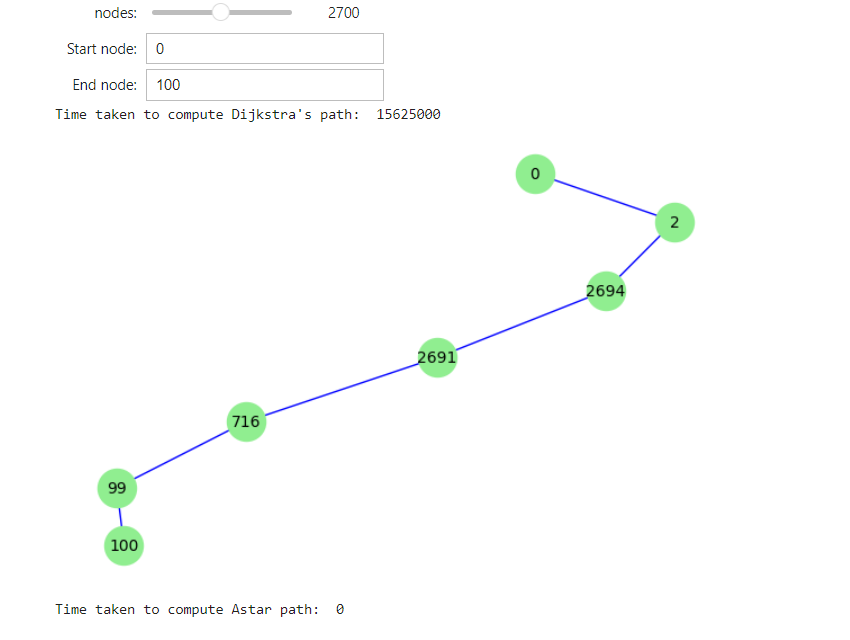
\includegraphics[keepaspectratio]{fig3.png}}
\pandocbounded{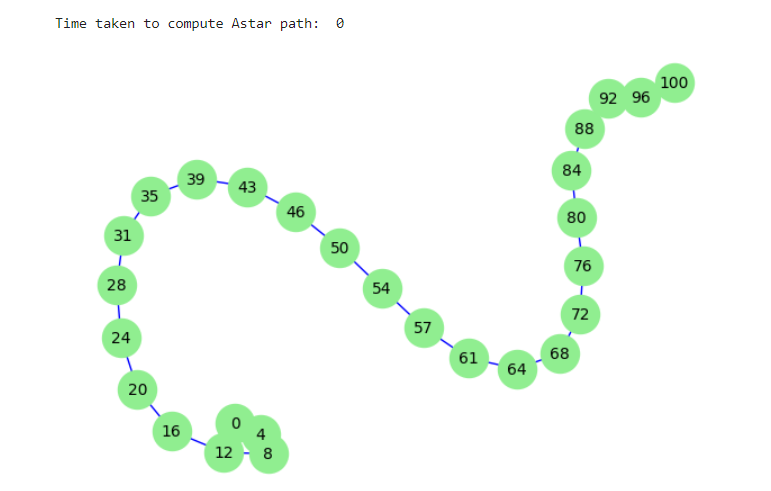
\includegraphics[keepaspectratio]{fig4.png}}

    \begin{enumerate}
\def\labelenumi{\arabic{enumi}.}
\setcounter{enumi}{1}
\tightlist
\item
  A* algorithm used in grids

  We will create a grid of size \(n\times n\), where you can choose the
  grid size \(n\), start node and end node to calculate shortest path.
  You can also add blocks in the grid. After placing blocks (if any),
  start and end nodes, just click calculate button to find the shortest
  path using A*. After the calculation, you can see green-colored cells
  in the grid which denotes the shortest path between start and end node
\end{enumerate}

    \begin{tcolorbox}[breakable, size=fbox, boxrule=1pt, pad at break*=1mm,colback=cellbackground, colframe=cellborder]
\prompt{In}{incolor}{ }{\boxspacing}
\begin{Verbatim}[commandchars=\\\{\}]
\PY{c+c1}{\PYZsh{} Initializing}
\PY{n}{canvas} \PY{o}{=} \PY{p}{[}\PY{p}{]}
\PY{n}{grid} \PY{o}{=} \PY{k+kc}{None}
\PY{n}{grid\PYZus{}size} \PY{o}{=} \PY{k+kc}{None}
\PY{n}{grid\PYZus{}graph} \PY{o}{=} \PY{k+kc}{None}
\PY{n}{cells} \PY{o}{=} \PY{k+kc}{None}
\PY{n}{block} \PY{o}{=} \PY{k+kc}{None}
\PY{n}{start} \PY{o}{=} \PY{k+kc}{None}
\PY{n}{end} \PY{o}{=} \PY{k+kc}{None}
\PY{n}{check\PYZus{}types} \PY{o}{=} \PY{p}{\PYZob{}}\PY{p}{\PYZcb{}}

\PY{c+c1}{\PYZsh{} Get grid size}
\PY{n}{inp\PYZus{}grid\PYZus{}size} \PY{o}{=} \PY{n}{widgets}\PY{o}{.}\PY{n}{IntText}\PY{p}{(}\PY{n}{description}\PY{o}{=}\PY{l+s+s1}{\PYZsq{}}\PY{l+s+s1}{size}\PY{l+s+s1}{\PYZsq{}}\PY{p}{,} \PY{n}{value}\PY{o}{=}\PY{l+m+mi}{5}\PY{p}{)}
\PY{n}{output} \PY{o}{=} \PY{n}{widgets}\PY{o}{.}\PY{n}{Output}\PY{p}{(}\PY{p}{)}

\PY{n}{canvas}\PY{o}{+}\PY{o}{=}\PY{p}{[}\PY{n}{inp\PYZus{}grid\PYZus{}size}\PY{p}{]}
\PY{c+c1}{\PYZsh{} Define heuristics function for a\PYZhy{}star search algorithm}
\PY{k}{def} \PY{n+nf}{heuristics}\PY{p}{(}\PY{n}{a}\PY{p}{,}\PY{n}{b}\PY{p}{)}\PY{p}{:}
    \PY{n}{x0}\PY{p}{,}\PY{n}{y0} \PY{o}{=} \PY{n+nb}{int}\PY{p}{(}\PY{n}{a}\PY{p}{[}\PY{l+m+mi}{0}\PY{p}{]}\PY{p}{)}\PY{p}{,} \PY{n+nb}{int}\PY{p}{(}\PY{n}{a}\PY{p}{[}\PY{l+m+mi}{1}\PY{p}{]}\PY{p}{)}
    \PY{n}{x1}\PY{p}{,}\PY{n}{y1} \PY{o}{=} \PY{n+nb}{int}\PY{p}{(}\PY{n}{b}\PY{p}{[}\PY{l+m+mi}{0}\PY{p}{]}\PY{p}{)}\PY{p}{,} \PY{n+nb}{int}\PY{p}{(}\PY{n}{b}\PY{p}{[}\PY{l+m+mi}{1}\PY{p}{]}\PY{p}{)}
    \PY{k}{return} \PY{p}{(}\PY{p}{(}\PY{n}{x1}\PY{o}{\PYZhy{}}\PY{n}{x0}\PY{p}{)}\PY{o}{*}\PY{o}{*}\PY{l+m+mi}{2} \PY{o}{+} \PY{p}{(}\PY{n}{y1}\PY{o}{\PYZhy{}}\PY{n}{y0}\PY{p}{)}\PY{o}{*}\PY{o}{*}\PY{l+m+mi}{2}\PY{p}{)}\PY{o}{*}\PY{o}{*}\PY{l+m+mf}{0.5}

\PY{k}{def} \PY{n+nf}{toggler}\PY{p}{(}\PY{n}{change}\PY{p}{)}\PY{p}{:}
    \PY{n}{owner\PYZus{}name} \PY{o}{=} \PY{n}{change}\PY{o}{.}\PY{n}{get}\PY{p}{(}\PY{l+s+s2}{\PYZdq{}}\PY{l+s+s2}{owner}\PY{l+s+s2}{\PYZdq{}}\PY{p}{,}\PY{p}{\PYZob{}}\PY{l+s+s2}{\PYZdq{}}\PY{l+s+s2}{description}\PY{l+s+s2}{\PYZdq{}}\PY{p}{:} \PY{l+s+s2}{\PYZdq{}}\PY{l+s+s2}{\PYZdq{}}\PY{p}{\PYZcb{}}\PY{p}{)}\PY{o}{.}\PY{n}{description}
    \PY{k}{for} \PY{n}{key} \PY{o+ow}{in} \PY{n}{check\PYZus{}types}\PY{o}{.}\PY{n}{keys}\PY{p}{(}\PY{p}{)}\PY{p}{:}
        \PY{k}{if} \PY{n}{key} \PY{o}{!=} \PY{n}{owner\PYZus{}name}\PY{p}{:}
            \PY{n}{check\PYZus{}types}\PY{p}{[}\PY{n}{key}\PY{p}{]}\PY{p}{[}\PY{l+s+s2}{\PYZdq{}}\PY{l+s+s2}{obj}\PY{l+s+s2}{\PYZdq{}}\PY{p}{]}\PY{o}{.}\PY{n}{value} \PY{o}{=} \PY{k+kc}{False}

\PY{k}{def} \PY{n+nf}{update\PYZus{}grid}\PY{p}{(}\PY{n}{widget}\PY{p}{)}\PY{p}{:}
    \PY{k}{global} \PY{n}{start\PYZus{}node}\PY{p}{,} \PY{n}{end\PYZus{}node}
    \PY{k}{if} \PY{p}{(}\PY{n}{widget}\PY{o}{.}\PY{n}{description} \PY{o}{==} \PY{l+s+s2}{\PYZdq{}}\PY{l+s+s2}{Calculate}\PY{l+s+s2}{\PYZdq{}}\PY{p}{)}\PY{p}{:}
        \PY{n}{start\PYZus{}time} \PY{o}{=} \PY{n}{time}\PY{o}{.}\PY{n}{process\PYZus{}time\PYZus{}ns}\PY{p}{(}\PY{p}{)}
        \PY{n}{astar\PYZus{}paths} \PY{o}{=} \PY{n}{nx}\PY{o}{.}\PY{n}{astar\PYZus{}path}\PY{p}{(}\PY{n}{grid\PYZus{}graph}\PY{p}{,} \PY{n}{start\PYZus{}node}\PY{p}{,} \PY{n}{end\PYZus{}node}\PY{p}{,} \PY{n}{heuristics}\PY{p}{)}
        \PY{n}{end\PYZus{}time} \PY{o}{=} \PY{n}{time}\PY{o}{.}\PY{n}{process\PYZus{}time\PYZus{}ns}\PY{p}{(}\PY{p}{)}
        \PY{k}{with} \PY{n}{output}\PY{p}{:}
            \PY{n+nb}{print}\PY{p}{(}\PY{l+s+s2}{\PYZdq{}}\PY{l+s+s2}{Time to calculate the path: }\PY{l+s+s2}{\PYZdq{}}\PY{p}{,} \PY{n}{end\PYZus{}time} \PY{o}{\PYZhy{}} \PY{n}{start\PYZus{}time}\PY{p}{)}
        \PY{c+c1}{\PYZsh{} Highlight paths of astar}
        \PY{k}{for} \PY{n}{node} \PY{o+ow}{in} \PY{n}{astar\PYZus{}paths}\PY{p}{[}\PY{l+m+mi}{1}\PY{p}{:}\PY{o}{\PYZhy{}}\PY{l+m+mi}{1}\PY{p}{]}\PY{p}{:}
            \PY{n}{i}\PY{p}{,}\PY{n}{j} \PY{o}{=} \PY{n}{node}\PY{p}{[}\PY{l+m+mi}{0}\PY{p}{]}\PY{p}{,} \PY{n}{node}\PY{p}{[}\PY{l+m+mi}{1}\PY{p}{]}
            \PY{n}{cells}\PY{p}{[}\PY{n}{i}\PY{p}{]}\PY{o}{.}\PY{n}{children}\PY{p}{[}\PY{n}{j}\PY{p}{]}\PY{o}{.}\PY{n}{style}\PY{o}{.}\PY{n}{button\PYZus{}color}\PY{o}{=}\PY{l+s+s2}{\PYZdq{}}\PY{l+s+s2}{green}\PY{l+s+s2}{\PYZdq{}}
             
    \PY{k}{else}\PY{p}{:}
        \PY{c+c1}{\PYZsh{} for cells}
        \PY{n}{x}\PY{p}{,}\PY{n}{y} \PY{o}{=} \PY{p}{[}\PY{n+nb}{int}\PY{p}{(}\PY{n}{i}\PY{p}{)} \PY{k}{for} \PY{n}{i} \PY{o+ow}{in} \PY{n}{widget}\PY{o}{.}\PY{n}{description}\PY{o}{.}\PY{n}{split}\PY{p}{(}\PY{l+s+s2}{\PYZdq{}}\PY{l+s+s2}{,}\PY{l+s+s2}{\PYZdq{}}\PY{p}{)}\PY{p}{]}
        \PY{n}{cell\PYZus{}type} \PY{o}{=} \PY{p}{[}\PY{n}{val} \PY{k}{for} \PY{n}{val} \PY{o+ow}{in} \PY{n}{check\PYZus{}types}\PY{o}{.}\PY{n}{values}\PY{p}{(}\PY{p}{)} \PY{k}{if} \PY{n}{val}\PY{p}{[}\PY{l+s+s2}{\PYZdq{}}\PY{l+s+s2}{obj}\PY{l+s+s2}{\PYZdq{}}\PY{p}{]}\PY{o}{.}\PY{n}{value}\PY{p}{]}
        \PY{k}{if} \PY{n}{cell\PYZus{}type}\PY{p}{:}
            \PY{n}{cell} \PY{o}{=} \PY{n}{cell\PYZus{}type}\PY{p}{[}\PY{l+m+mi}{0}\PY{p}{]}
            \PY{k}{if} \PY{n}{cell}\PY{p}{[}\PY{l+s+s2}{\PYZdq{}}\PY{l+s+s2}{ops}\PY{l+s+s2}{\PYZdq{}}\PY{p}{]} \PY{o}{==} \PY{l+s+s2}{\PYZdq{}}\PY{l+s+s2}{remove\PYZus{}cell}\PY{l+s+s2}{\PYZdq{}}\PY{p}{:}
                \PY{k}{if} \PY{n}{cell}\PY{p}{[}\PY{l+s+s2}{\PYZdq{}}\PY{l+s+s2}{color}\PY{l+s+s2}{\PYZdq{}}\PY{p}{]} \PY{o}{==} \PY{n}{widget}\PY{o}{.}\PY{n}{style}\PY{o}{.}\PY{n}{button\PYZus{}color}\PY{p}{:}
                    \PY{n}{edges} \PY{o}{=} \PY{p}{[}\PY{p}{(}\PY{p}{(}\PY{n}{x}\PY{o}{\PYZhy{}}\PY{n}{i}\PY{p}{,}\PY{n}{y}\PY{o}{\PYZhy{}}\PY{n}{j}\PY{p}{)}\PY{p}{,}\PY{p}{(}\PY{n}{x}\PY{p}{,}\PY{n}{y}\PY{p}{)}\PY{p}{)} \PY{k}{for} \PY{p}{(}\PY{n}{i}\PY{p}{,}\PY{n}{j}\PY{p}{)} \PY{o+ow}{in} \PY{p}{[}\PY{p}{(}\PY{l+m+mi}{0}\PY{p}{,}\PY{l+m+mi}{1}\PY{p}{)}\PY{p}{,}\PY{p}{(}\PY{l+m+mi}{1}\PY{p}{,}\PY{l+m+mi}{0}\PY{p}{)}\PY{p}{,} \PY{p}{(}\PY{l+m+mi}{0}\PY{p}{,}\PY{o}{\PYZhy{}}\PY{l+m+mi}{1}\PY{p}{)}\PY{p}{,} \PY{p}{(}\PY{o}{\PYZhy{}}\PY{l+m+mi}{1}\PY{p}{,}\PY{l+m+mi}{0}\PY{p}{)}\PY{p}{,} \PY{p}{(}\PY{l+m+mi}{1}\PY{p}{,}\PY{l+m+mi}{1}\PY{p}{)}\PY{p}{,}\PY{p}{(}\PY{l+m+mi}{1}\PY{p}{,}\PY{o}{\PYZhy{}}\PY{l+m+mi}{1}\PY{p}{)}\PY{p}{,} \PY{p}{(}\PY{o}{\PYZhy{}}\PY{l+m+mi}{1}\PY{p}{,}\PY{o}{\PYZhy{}}\PY{l+m+mi}{1}\PY{p}{)}\PY{p}{,} \PY{p}{(}\PY{o}{\PYZhy{}}\PY{l+m+mi}{1}\PY{p}{,}\PY{l+m+mi}{1}\PY{p}{)}\PY{p}{]} \PY{k}{if} \PY{p}{(}\PY{l+m+mi}{0}\PY{o}{\PYZlt{}}\PY{o}{=}\PY{p}{(}\PY{n}{x}\PY{o}{\PYZhy{}}\PY{n}{i}\PY{p}{)}\PY{o}{\PYZlt{}}\PY{n}{grid\PYZus{}size}\PY{p}{)} \PY{o+ow}{and} \PY{p}{(}\PY{l+m+mi}{0}\PY{o}{\PYZlt{}}\PY{o}{=}\PY{p}{(}\PY{n}{y}\PY{o}{\PYZhy{}}\PY{n}{j}\PY{p}{)}\PY{o}{\PYZlt{}}\PY{n}{grid\PYZus{}size}\PY{p}{)}\PY{p}{]}
                    \PY{n}{grid\PYZus{}graph}\PY{o}{.}\PY{n}{add\PYZus{}edges\PYZus{}from}\PY{p}{(}\PY{n}{edges}\PY{p}{)}
                    \PY{n}{widget}\PY{o}{.}\PY{n}{style}\PY{o}{.}\PY{n}{button\PYZus{}color} \PY{o}{=} \PY{l+s+s2}{\PYZdq{}}\PY{l+s+s2}{lightgrey}\PY{l+s+s2}{\PYZdq{}}
                    \PY{k}{return}
                \PY{n}{grid\PYZus{}graph}\PY{o}{.}\PY{n}{remove\PYZus{}node}\PY{p}{(}\PY{p}{(}\PY{n}{x}\PY{p}{,}\PY{n}{y}\PY{p}{)}\PY{p}{)}
            \PY{k}{elif} \PY{n}{cell}\PY{p}{[}\PY{l+s+s2}{\PYZdq{}}\PY{l+s+s2}{ops}\PY{l+s+s2}{\PYZdq{}}\PY{p}{]} \PY{o}{==} \PY{l+s+s2}{\PYZdq{}}\PY{l+s+s2}{set\PYZus{}start\PYZus{}node}\PY{l+s+s2}{\PYZdq{}}\PY{p}{:}
                \PY{n}{start\PYZus{}node} \PY{o}{=} \PY{p}{(}\PY{n}{x}\PY{p}{,}\PY{n}{y}\PY{p}{)}
            \PY{k}{elif} \PY{n}{cell}\PY{p}{[}\PY{l+s+s2}{\PYZdq{}}\PY{l+s+s2}{ops}\PY{l+s+s2}{\PYZdq{}}\PY{p}{]} \PY{o}{==} \PY{l+s+s2}{\PYZdq{}}\PY{l+s+s2}{set\PYZus{}end\PYZus{}node}\PY{l+s+s2}{\PYZdq{}}\PY{p}{:}
                \PY{n}{end\PYZus{}node} \PY{o}{=} \PY{p}{(}\PY{n}{x}\PY{p}{,}\PY{n}{y}\PY{p}{)}
            \PY{n}{widget}\PY{o}{.}\PY{n}{style}\PY{o}{.}\PY{n}{button\PYZus{}color} \PY{o}{=} \PY{n}{cell}\PY{p}{[}\PY{l+s+s2}{\PYZdq{}}\PY{l+s+s2}{color}\PY{l+s+s2}{\PYZdq{}}\PY{p}{]}
            \PY{k}{return}
        \PY{n}{widget}\PY{o}{.}\PY{n}{style}\PY{o}{.}\PY{n}{button\PYZus{}color} \PY{o}{=} \PY{l+s+s2}{\PYZdq{}}\PY{l+s+s2}{lightgrey}\PY{l+s+s2}{\PYZdq{}}


\PY{k}{def} \PY{n+nf}{reset}\PY{p}{(}\PY{n}{\PYZus{}}\PY{p}{)}\PY{p}{:}
    \PY{n}{create\PYZus{}grid}\PY{p}{(}\PY{p}{)}

\PY{k}{def} \PY{n+nf}{create\PYZus{}grid}\PY{p}{(}\PY{n}{change}\PY{o}{=}\PY{k+kc}{None}\PY{p}{)}\PY{p}{:}
    \PY{k}{global} \PY{n}{grid\PYZus{}graph}\PY{p}{,} \PY{n}{cells}\PY{p}{,} \PY{n}{grid\PYZus{}size}
    \PY{n}{grid\PYZus{}size} \PY{o}{=} \PY{n}{inp\PYZus{}grid\PYZus{}size}\PY{o}{.}\PY{n}{get\PYZus{}interact\PYZus{}value}\PY{p}{(}\PY{p}{)}
    \PY{c+c1}{\PYZsh{} Creating graph with edges that is similar to functions used in a grid to move from one cell to another}
    \PY{n}{grid\PYZus{}graph} \PY{o}{=} \PY{n}{nx}\PY{o}{.}\PY{n}{grid\PYZus{}graph}\PY{p}{(}\PY{p}{(}\PY{n}{grid\PYZus{}size}\PY{p}{,}\PY{n}{grid\PYZus{}size}\PY{p}{)}\PY{p}{)}
    \PY{k}{for} \PY{n}{node} \PY{o+ow}{in} \PY{n}{grid\PYZus{}graph}\PY{o}{.}\PY{n}{nodes}\PY{p}{(}\PY{p}{)}\PY{p}{:}
        \PY{n}{x}\PY{p}{,}\PY{n}{y} \PY{o}{=} \PY{n}{node}
        \PY{c+c1}{\PYZsh{} Adding diagonal connections}
        \PY{n}{edges} \PY{o}{=} \PY{p}{[}\PY{p}{(}\PY{p}{(}\PY{n}{x}\PY{o}{\PYZhy{}}\PY{n}{i}\PY{p}{,}\PY{n}{y}\PY{o}{\PYZhy{}}\PY{n}{j}\PY{p}{)}\PY{p}{,}\PY{p}{(}\PY{n}{x}\PY{p}{,}\PY{n}{y}\PY{p}{)}\PY{p}{)} \PY{k}{for} \PY{p}{(}\PY{n}{i}\PY{p}{,}\PY{n}{j}\PY{p}{)} \PY{o+ow}{in} \PY{p}{[}\PY{p}{(}\PY{l+m+mi}{1}\PY{p}{,}\PY{l+m+mi}{1}\PY{p}{)}\PY{p}{,}\PY{p}{(}\PY{l+m+mi}{1}\PY{p}{,}\PY{o}{\PYZhy{}}\PY{l+m+mi}{1}\PY{p}{)}\PY{p}{,} \PY{p}{(}\PY{o}{\PYZhy{}}\PY{l+m+mi}{1}\PY{p}{,}\PY{o}{\PYZhy{}}\PY{l+m+mi}{1}\PY{p}{)}\PY{p}{,} \PY{p}{(}\PY{o}{\PYZhy{}}\PY{l+m+mi}{1}\PY{p}{,}\PY{l+m+mi}{1}\PY{p}{)}\PY{p}{]} \PY{k}{if} \PY{p}{(}\PY{l+m+mi}{0}\PY{o}{\PYZlt{}}\PY{o}{=}\PY{p}{(}\PY{n}{x}\PY{o}{\PYZhy{}}\PY{n}{i}\PY{p}{)}\PY{o}{\PYZlt{}}\PY{n}{grid\PYZus{}size}\PY{p}{)} \PY{o+ow}{and} \PY{p}{(}\PY{l+m+mi}{0}\PY{o}{\PYZlt{}}\PY{o}{=}\PY{p}{(}\PY{n}{y}\PY{o}{\PYZhy{}}\PY{n}{j}\PY{p}{)}\PY{o}{\PYZlt{}}\PY{n}{grid\PYZus{}size}\PY{p}{)}\PY{p}{]}
        \PY{n}{grid\PYZus{}graph}\PY{o}{.}\PY{n}{add\PYZus{}edges\PYZus{}from}\PY{p}{(}\PY{n}{edges}\PY{p}{)}
    \PY{k}{with} \PY{n}{output}\PY{p}{:}
        \PY{n}{output}\PY{o}{.}\PY{n}{clear\PYZus{}output}\PY{p}{(}\PY{n}{wait}\PY{o}{=}\PY{k+kc}{True}\PY{p}{)}
        \PY{n}{plot\PYZus{}canvas} \PY{o}{=} \PY{p}{[}\PY{p}{]}
        \PY{n}{cells} \PY{o}{=} \PY{p}{[}\PY{p}{]}
        \PY{k}{for} \PY{n}{i} \PY{o+ow}{in} \PY{n+nb}{range}\PY{p}{(}\PY{n}{grid\PYZus{}size}\PY{p}{)}\PY{p}{:}
            \PY{n}{row} \PY{o}{=} \PY{p}{[}\PY{p}{]}
            \PY{k}{for} \PY{n}{j} \PY{o+ow}{in} \PY{n+nb}{range}\PY{p}{(}\PY{n}{grid\PYZus{}size}\PY{p}{)}\PY{p}{:}
                \PY{c+c1}{\PYZsh{} Creating button as a cell}
                \PY{n}{cell} \PY{o}{=} \PY{n}{widgets}\PY{o}{.}\PY{n}{Button}\PY{p}{(}
                    \PY{n}{description}\PY{o}{=}\PY{l+s+sa}{f}\PY{l+s+s2}{\PYZdq{}}\PY{l+s+si}{\PYZob{}}\PY{n}{i}\PY{l+s+si}{\PYZcb{}}\PY{l+s+s2}{,}\PY{l+s+si}{\PYZob{}}\PY{n}{j}\PY{l+s+si}{\PYZcb{}}\PY{l+s+s2}{\PYZdq{}}\PY{p}{,}  
                    \PY{n}{layout}\PY{o}{=}\PY{n}{widgets}\PY{o}{.}\PY{n}{Layout}\PY{p}{(}\PY{n}{width}\PY{o}{=}\PY{l+s+s1}{\PYZsq{}}\PY{l+s+s1}{20px}\PY{l+s+s1}{\PYZsq{}}\PY{p}{,} \PY{n}{height}\PY{o}{=}\PY{l+s+s1}{\PYZsq{}}\PY{l+s+s1}{20px}\PY{l+s+s1}{\PYZsq{}}\PY{p}{)}\PY{p}{,}
                    \PY{n}{style}\PY{o}{=}\PY{n}{widgets}\PY{o}{.}\PY{n}{ButtonStyle}\PY{p}{(}\PY{n}{font\PYZus{}size}\PY{o}{=}\PY{l+s+s2}{\PYZdq{}}\PY{l+s+s2}{10px}\PY{l+s+s2}{\PYZdq{}}\PY{p}{,} \PY{n}{button\PYZus{}color}\PY{o}{=}\PY{l+s+s2}{\PYZdq{}}\PY{l+s+s2}{lightgrey}\PY{l+s+s2}{\PYZdq{}}\PY{p}{)}
                    \PY{p}{)} 
                \PY{n}{cell}\PY{o}{.}\PY{n}{on\PYZus{}click}\PY{p}{(}\PY{n}{update\PYZus{}grid}\PY{p}{)}
                \PY{n}{row}\PY{o}{.}\PY{n}{append}\PY{p}{(}\PY{n}{cell}\PY{p}{)}
            \PY{n}{cells}\PY{o}{.}\PY{n}{append}\PY{p}{(}\PY{n}{widgets}\PY{o}{.}\PY{n}{HBox}\PY{p}{(}\PY{n}{row}\PY{p}{)}\PY{p}{)}
        \PY{n}{plot\PYZus{}canvas}\PY{o}{.}\PY{n}{append}\PY{p}{(}\PY{n}{widgets}\PY{o}{.}\PY{n}{VBox}\PY{p}{(}\PY{n}{cells}\PY{p}{)}\PY{p}{)}
        
        \PY{c+c1}{\PYZsh{} Blocks}
        \PY{n}{block} \PY{o}{=} \PY{n}{widgets}\PY{o}{.}\PY{n}{Checkbox}\PY{p}{(}\PY{n}{description}\PY{o}{=}\PY{l+s+s2}{\PYZdq{}}\PY{l+s+s2}{Add Block}\PY{l+s+s2}{\PYZdq{}}\PY{p}{)}
        \PY{n}{block}\PY{o}{.}\PY{n}{observe}\PY{p}{(}\PY{n}{toggler}\PY{p}{)}
        \PY{n}{check\PYZus{}types}\PY{p}{[}\PY{l+s+s2}{\PYZdq{}}\PY{l+s+s2}{Add Block}\PY{l+s+s2}{\PYZdq{}}\PY{p}{]} \PY{o}{=} \PY{p}{\PYZob{}}\PY{l+s+s2}{\PYZdq{}}\PY{l+s+s2}{obj}\PY{l+s+s2}{\PYZdq{}}\PY{p}{:} \PY{n}{block}\PY{p}{,} \PY{l+s+s2}{\PYZdq{}}\PY{l+s+s2}{color}\PY{l+s+s2}{\PYZdq{}}\PY{p}{:} \PY{l+s+s2}{\PYZdq{}}\PY{l+s+s2}{black}\PY{l+s+s2}{\PYZdq{}}\PY{p}{,} \PY{l+s+s2}{\PYZdq{}}\PY{l+s+s2}{ops}\PY{l+s+s2}{\PYZdq{}}\PY{p}{:} \PY{l+s+s2}{\PYZdq{}}\PY{l+s+s2}{remove\PYZus{}cell}\PY{l+s+s2}{\PYZdq{}}\PY{p}{\PYZcb{}}
        \PY{c+c1}{\PYZsh{} start node}
        \PY{n}{start\PYZus{}node\PYZus{}inp} \PY{o}{=} \PY{n}{widgets}\PY{o}{.}\PY{n}{Checkbox}\PY{p}{(}\PY{n}{description}\PY{o}{=}\PY{l+s+s2}{\PYZdq{}}\PY{l+s+s2}{Start Node}\PY{l+s+s2}{\PYZdq{}}\PY{p}{)}
        \PY{n}{start\PYZus{}node\PYZus{}inp}\PY{o}{.}\PY{n}{observe}\PY{p}{(}\PY{n}{toggler}\PY{p}{)}
        \PY{n}{check\PYZus{}types}\PY{p}{[}\PY{l+s+s2}{\PYZdq{}}\PY{l+s+s2}{Start Node}\PY{l+s+s2}{\PYZdq{}}\PY{p}{]} \PY{o}{=} \PY{p}{\PYZob{}}\PY{l+s+s2}{\PYZdq{}}\PY{l+s+s2}{obj}\PY{l+s+s2}{\PYZdq{}}\PY{p}{:} \PY{n}{start\PYZus{}node\PYZus{}inp}\PY{p}{,} \PY{l+s+s2}{\PYZdq{}}\PY{l+s+s2}{color}\PY{l+s+s2}{\PYZdq{}}\PY{p}{:} \PY{l+s+s2}{\PYZdq{}}\PY{l+s+s2}{blue}\PY{l+s+s2}{\PYZdq{}}\PY{p}{,} \PY{l+s+s2}{\PYZdq{}}\PY{l+s+s2}{ops}\PY{l+s+s2}{\PYZdq{}}\PY{p}{:} \PY{l+s+s2}{\PYZdq{}}\PY{l+s+s2}{set\PYZus{}start\PYZus{}node}\PY{l+s+s2}{\PYZdq{}}\PY{p}{\PYZcb{}}
        \PY{c+c1}{\PYZsh{} end node}
        \PY{n}{end\PYZus{}node\PYZus{}inp} \PY{o}{=} \PY{n}{widgets}\PY{o}{.}\PY{n}{Checkbox}\PY{p}{(}\PY{n}{description}\PY{o}{=}\PY{l+s+s2}{\PYZdq{}}\PY{l+s+s2}{End Node}\PY{l+s+s2}{\PYZdq{}}\PY{p}{)}
        \PY{n}{end\PYZus{}node\PYZus{}inp}\PY{o}{.}\PY{n}{observe}\PY{p}{(}\PY{n}{toggler}\PY{p}{)}
        \PY{n}{check\PYZus{}types}\PY{p}{[}\PY{l+s+s2}{\PYZdq{}}\PY{l+s+s2}{End Node}\PY{l+s+s2}{\PYZdq{}}\PY{p}{]} \PY{o}{=} \PY{p}{\PYZob{}}\PY{l+s+s2}{\PYZdq{}}\PY{l+s+s2}{obj}\PY{l+s+s2}{\PYZdq{}}\PY{p}{:} \PY{n}{end\PYZus{}node\PYZus{}inp}\PY{p}{,} \PY{l+s+s2}{\PYZdq{}}\PY{l+s+s2}{color}\PY{l+s+s2}{\PYZdq{}}\PY{p}{:} \PY{l+s+s2}{\PYZdq{}}\PY{l+s+s2}{red}\PY{l+s+s2}{\PYZdq{}}\PY{p}{,} \PY{l+s+s2}{\PYZdq{}}\PY{l+s+s2}{ops}\PY{l+s+s2}{\PYZdq{}}\PY{p}{:} \PY{l+s+s2}{\PYZdq{}}\PY{l+s+s2}{set\PYZus{}end\PYZus{}node}\PY{l+s+s2}{\PYZdq{}}\PY{p}{\PYZcb{}}
        \PY{c+c1}{\PYZsh{} Calculate distance}
        \PY{n}{calc\PYZus{}btn} \PY{o}{=} \PY{n}{widgets}\PY{o}{.}\PY{n}{Button}\PY{p}{(}\PY{n}{description}\PY{o}{=}\PY{l+s+s2}{\PYZdq{}}\PY{l+s+s2}{Calculate}\PY{l+s+s2}{\PYZdq{}}\PY{p}{)}
        \PY{n}{calc\PYZus{}btn}\PY{o}{.}\PY{n}{on\PYZus{}click}\PY{p}{(}\PY{n}{update\PYZus{}grid}\PY{p}{)}
        \PY{c+c1}{\PYZsh{} Reset entire grid}
        \PY{n}{reset\PYZus{}btn} \PY{o}{=} \PY{n}{widgets}\PY{o}{.}\PY{n}{Button}\PY{p}{(}\PY{n}{description}\PY{o}{=}\PY{l+s+s2}{\PYZdq{}}\PY{l+s+s2}{Reset}\PY{l+s+s2}{\PYZdq{}}\PY{p}{)}
        \PY{n}{reset\PYZus{}btn}\PY{o}{.}\PY{n}{on\PYZus{}click}\PY{p}{(}\PY{n}{reset}\PY{p}{)}
        \PY{c+c1}{\PYZsh{} Add it to canvas plot}
        \PY{n}{plot\PYZus{}canvas} \PY{o}{.}\PY{n}{append}\PY{p}{(}\PY{n}{widgets}\PY{o}{.}\PY{n}{VBox}\PY{p}{(}\PY{p}{[}\PY{n}{block}\PY{p}{,} \PY{n}{start\PYZus{}node\PYZus{}inp}\PY{p}{,} \PY{n}{end\PYZus{}node\PYZus{}inp}\PY{p}{,} \PY{n}{calc\PYZus{}btn}\PY{p}{,}\PY{n}{reset\PYZus{}btn}\PY{p}{]}\PY{p}{)}\PY{p}{)}
        \PY{n}{display}\PY{p}{(}\PY{n}{widgets}\PY{o}{.}\PY{n}{HBox}\PY{p}{(}\PY{n}{plot\PYZus{}canvas}\PY{p}{)}\PY{p}{)}          

\PY{n}{inp\PYZus{}grid\PYZus{}size}\PY{o}{.}\PY{n}{observe}\PY{p}{(}\PY{n}{create\PYZus{}grid}\PY{p}{,} \PY{n}{names}\PY{o}{=}\PY{l+s+s2}{\PYZdq{}}\PY{l+s+s2}{value}\PY{l+s+s2}{\PYZdq{}}\PY{p}{)}
\PY{n}{display}\PY{p}{(}\PY{n}{widgets}\PY{o}{.}\PY{n}{HBox}\PY{p}{(}\PY{n}{canvas}\PY{p}{)}\PY{p}{,} \PY{n}{output}\PY{p}{)}
\PY{n}{create\PYZus{}grid}\PY{p}{(}\PY{p}{)}
\end{Verbatim}
\end{tcolorbox}

    Observation

For below state of the grid:

Grid size: \(5 \times 5\)

Blocks are placed at: \((2,1), (2,2), (1,2)\)

Start Node: \((0,0)\)

End Node: \((3,3)\)

After calculating the shortest path:

\begin{figure}
\centering
\pandocbounded{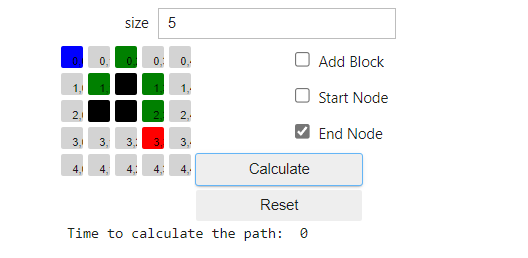
\includegraphics[keepaspectratio]{fig5.png}}
\caption{title}
\end{figure}

The reason for selecting \((1,1)\) as the first cell in the shortest
path is because the value of heuristic function evaluated at \((1,1)\)
is lesser compared to other cells \((1,0), (0,1)\).

Since
\(Heuristics((x_0, y_0), (x_1, y_1)) = \sqrt{(x_0 - x_1)^2+(y_0 - y_1)^2}\)

\(Heuristics((1,1),(3,3)) = 2.83\)

\(Heuristics((1,0),(3,3)) = 3.61\)

\(Heuristics((0,1),(3,3)) = 3.61\)

    Other Search Algorithms (Vishal Thomas 1234108347)

Dijkstra's Algorithm\(^{[4]}\)

An algorithm to find the shortest path in a graph with positive edge
weights. It maintains a set of visited and unvisited vertices. It moves
to next unvisited node from a node and update the distance if its lower
than the preivous. This process continue until the destination vertex is
reached.

Greedy Best First Search\(^{[5]}\)

A pathfinding algorithm that works by utilising heuristic function to
determine cost effective paths. It identifies the shortest path by
evaluating the heuristic function from the current node to the end node.
This process is continued until destination node is reached.

Bellman-Ford Algorithm\(^{[6]}\)

It is a shortest path algorithm which works well in negative weighted
edges. It updates the shortest distance of node, if a shorter path is
found through another node.

Floyd-Warshall Algorithm\(^{[7]}\)

It's the shortest path finding algorithm for all pairs of vertices. For
reducing time complexity, it uses Dynamic Programming approach to find
the shortest path between vertices, if possible. It doesn't work for
negative cycles, where your sum of edges in a cycle is less than zero.

Comparisons (Vishal Thomas 1234108347)

For understanding how A* algorithm differs from above mentioned path
finding algorithms, we are using certain features to differ them, such
as:

Optimization: Discuss on what area algorithm is optimized for.\(^{[4]}\)

Greedy Best First Search: Finding shortest path between single source
node and all other nodes based on heuristic function that depends on
current node and end node.

Dijkstra's Algorithm: Finding shortest path between single source node
and all other nodes with positive weighted edges.

Bellman-Ford Algorithm: Finding shortest path between single source node
and all other nodes including negative weighted edges.

Floyd-Warshall Algorithm: Finding shortest path between all pairs of
nodes with only positive weighted edges.

A* Algorithm: Finding shortest path between start and end nodes by
reducing search space

\begin{verbatim}
</li>
<li><b>Relaxation</b>: Discuss on how weights are updated in each iteration.$^{[4]}$
    <ol>
    <li><b>Greedy Best First Search</b>: It finds the node having the smallest distance in a greedy approach and updates the distance of its neighbours.</li>
    <li><b>Dijkstra's Algorithm</b>: It finds the node having the smallest distance based on the actual cost and updates the distance of its neighbours.</li>
    <li><b>Bellman-Ford Algorithm, Floyd-Warshall Algorithm</b>: It considers all possible paths to nodes and updates the distance of each node.</li>
    <li><b>A* Algorithm</b>: It chooses the node having minimal sum of distance from start node and heuristic distance from end node. Weights are updated after adding heuristics.</li>
    </ol>
</li>
<li><b>Time Complexity</b>: Discuss about the time taken by algorithm to complete. For below, $E$ stands for edges in the graph and $V$ stands for vertices in the graph.$^{[4]}$
    <ol>
    <li><b>Greedy Best First Search</b>: It depends on heuristic function.</li>
    <li><b>Dijkstra's Algorithm</b>: Average is <b>$O(E \times log(V))$</b>, worst is <b>$O(V^2)$</b>. </li>
    <li><b>Bellman-Ford Algorithm</b>: It has a time complexity of <b>$O(VE)$</b>.</li>
    <li><b>Floyd-Warshall Algorithm</b>: It has time complexity of $O(V^3)$.</li>
    <li><b>A* Algorithm</b>: Time complexity depends on heuristic function.</li>
    </ol>
</li>
<li><b>Search Techniques</b>: Discuss about the search techniques such as the parameters involved in updating weight functions.$^{[4]}$
    <ol>
    <li><b>Greedy Best First Search</b>: It uses heuristic function to reach to the end node.</li>
    <li><b>Dijkstra's Algorithm, Bellman-Ford Algorithm, Floyd-Warshall Algorithm</b>: It uses the weights initialized in the graph for calculating the shortest path.</li>
        <li><b>A* Algorithm</b>: It uses weights initialised and heuristic function to guide the search to end node</li>
    </ol>
</li>
\end{verbatim}

    \subsection{Variants (Vishal Thomas
124108347)}\label{variants-vishal-thomas-124108347}

Heirarchical Pathfinding A* (HPA*) .\(^{[3]}\)

Using hierarchical A\emph{, we can reduce the search space
hierarchically. For example, if we are going to Blackrock, Dublin from
Kinsale, Cork (as shown in Fig 2.), by using A} implementation we will
find all the cities in each county as nodes and find its heuristic
function value to compute the shortest path between these two. If we use
hierarchical A* algorithm, we can reduce the size of search space by
considering its counties as its nodes, not the cities. First travel to
the neighbourhood of the starting node i.e.~boundary of Cork County.
Then find the neighbourhood of the end node which is Dublin. After
reaching the neighbourhood, travel to the end node i.e.~Blackrock. As
you can see we have eliminated the cities(nodes) that are not part of
Cork and Dublin, and thus reduced search space dramatically resulting in
higher efficiency.

\begin{figure}
\centering
\pandocbounded{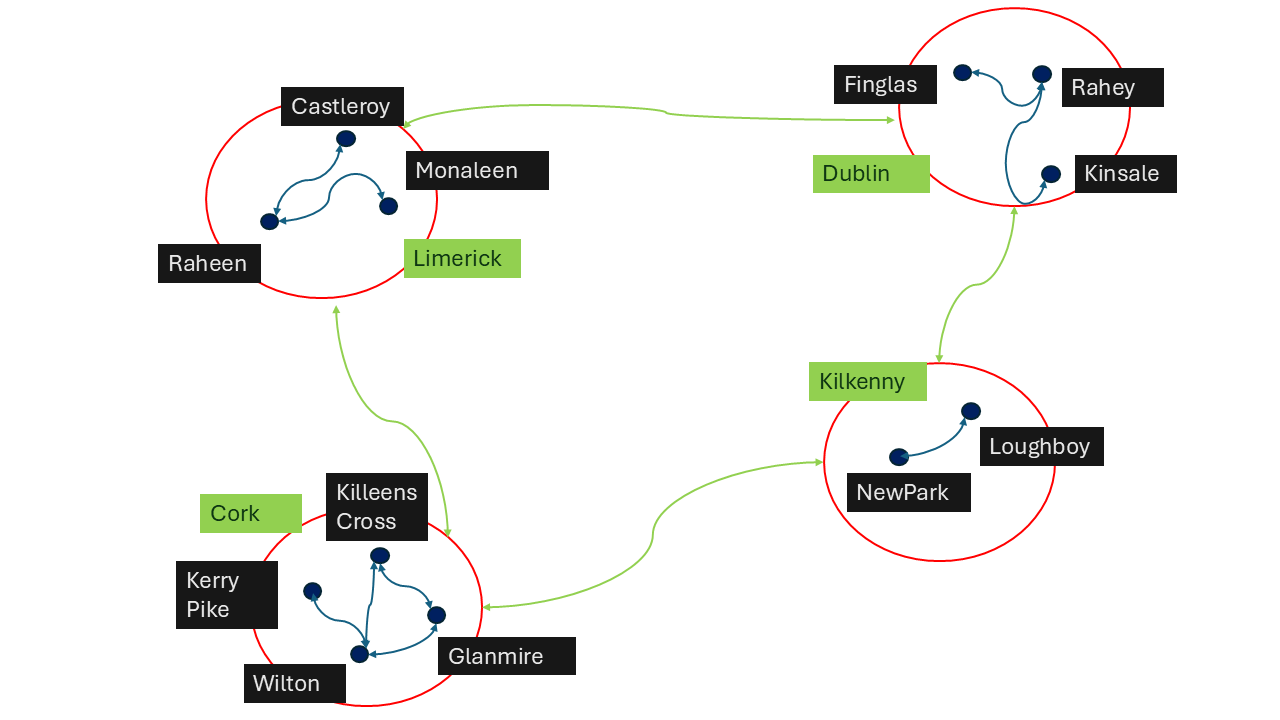
\includegraphics[keepaspectratio]{fig2.png}}
\caption{title}
\end{figure}

Fig 2: Red lined circles can be denoted as boundaries of start and end
nodes

    \subsection{Conclusions (Daniel Sedlov
123120712)}\label{conclusions-daniel-sedlov-123120712}

Few things in the world of computer science have as ubiquitous a
solution as pathfinding does. One look at any common problem such as
sorting, encryption, data transfer, or even machine learning will yield
dozens if not more of solutions and techniques all suggesting they each
be applied at different times in different situations to achieve
different results with different compromises.

While there might be small variations depending on the needs of the
user, overall,the core idea is the same. It is fast, efficient, and easy
to implement.

The A* algorithm is a unicorn in that it is quite commonly used as the
go-to pathfinding algorithm regardless of the scale, or application. It
is widely used in robotics and video games, such as the Unity Game
Engine (Unity Technologies. (n.d.)), where every millisecond is crucial,
and navigational software where finding the most efficient route is the
entire function. It is truly a jack of all trades.

    \subsection{References (Vishal Thomas
124108347)}\label{references-vishal-thomas-124108347}

{[}1{]}
https://www.geeksforgeeks.org/a-algorithm-and-its-heuristic-search-strategy-in-artificial-intelligence/
{[}2 {]}https://en.wikipedia.org/wiki/A*\_search\_algorithm {[}3{]} Cui,
Xiao \& Shi, Hao. A*-based Pathfinding in Modern Computer Games.
International journal of computer science and network security,
2011,11(1):125-130 {[}4{]}
https://www.geeksforgeeks.org/introduction-to-dijkstras-shortest-path-algorithm/
{[}5{]}
https://www.geeksforgeeks.org/greedy-best-first-search-algorithm/
{[}6{]} https://www.geeksforgeeks.org/bellman-ford-algorithm-dp-23/
{[}7{]} https://www.geeksforgeeks.org/floyd-warshall-algorithm-dp-16/

    \subsection{References (Daniel Sedlov
123120712)}\label{references-daniel-sedlov-123120712}

Goldstein, A. (1991, July 25). Oral-history:Bertram Raphael. ETHW.
https://ethw.org/Oral-History:Bertram\_Raphael

DARPA. (n.d.). Shakey the Robot. DARPA RSS.
https://www.darpa.mil/about-us/timeline/shakey-the-robot

Nilsson, N. J. (2013). The quest for artificial intelligence A history
of ideas and achievements Nils J. Nilsson. Cambridge Univ. Press. 12.1.1
https://ai.stanford.edu/\textasciitilde nilsson/QAI/qai.pdf

Patel, A. J. (2014, May 26). Introduction to A\emph{. Introduction to
the A} Algorithm.
https://www.redblobgames.com/pathfinding/a-star/introduction.html

Patel, A. J. (2014, July). Introduction to A\emph{. Implementation the
A} Algorithm.
https://www.redblobgames.com/pathfinding/a-star/implementation.html

Unity Technologies. (n.d.). Navigation areas and costs.
https://docs.unity3d.com/550/Documentation/Manual/nav-AreasAndCosts.html

    \begin{tcolorbox}[breakable, size=fbox, boxrule=1pt, pad at break*=1mm,colback=cellbackground, colframe=cellborder]
\prompt{In}{incolor}{ }{\boxspacing}
\begin{Verbatim}[commandchars=\\\{\}]

\end{Verbatim}
\end{tcolorbox}


    % Add a bibliography block to the postdoc
    
    
    
\end{document}
